
\documentclass[a4paper, 11pt]{article}
\author{Kajetan Kaczmarek}
\usepackage{amsmath}
\usepackage{subcaption}
\usepackage{mwe}
\usepackage{graphicx}
\usepackage{listings}
\usepackage[T1]{fontenc}
\usepackage[utf8]{inputenc}
\usepackage[polish]{babel}
\usepackage{color} %red, green, blue, yellow, cyan, magenta, black, white
\definecolor{mygreen}{RGB}{28,172,0} % color values Red, Green, Blue
\definecolor{mylilas}{RGB}{170,55,241}
\graphicspath{{Resources/}} %Setting the graphicspath
\usepackage{float}
%\usepackage[caption = false]{subfig}

\lstset{language=Matlab,%
    %basicstyle=\color{red},
      inputencoding=latin1,
    breaklines=true,%
    morekeywords={matlab2tikz},
    keywordstyle=\color{blue},%
    morekeywords=[2]{1}, keywordstyle=[2]{\color{black}},
    identifierstyle=\color{black},%
    stringstyle=\color{mylilas},
    commentstyle=\color{mygreen},%
    showstringspaces=false,%without this there will be a symbol in the places where there is a space
    basicstyle = \tiny,%
    numbers=left,%
    numberstyle={\tiny \color{black}},% size of the numbers
    numbersep=9pt, % this defines how far the numbers are from the text
    emph=[1]{for,end,break},emphstyle=[1]\color{red}, %some words to emphasise
    %emph=[2]{word1,word2}, emphstyle=[2]{style},    
}



\begin{document}
\title{Sprawozdanie STP \\* Projekt nr.2 \\* 
Zadanie 9 \\*}
\maketitle
\begin{enumerate}
\item Wyznaczamy modele w postaci : \\*
\[  y(k) = b_{\tau}u(k-\tau) +  b_{\tau+1}u(k-\tau -1) -a_1y(k-1)-a_2y(k-2)  \]
Gdzie \(\tau\) to opóźnienie systemu.
Wybrałem model dla \(\tau = 3\), wykres wyjścia modelu w porównaniu do danych z pliku : 
\begin{figure} [h]
\centering
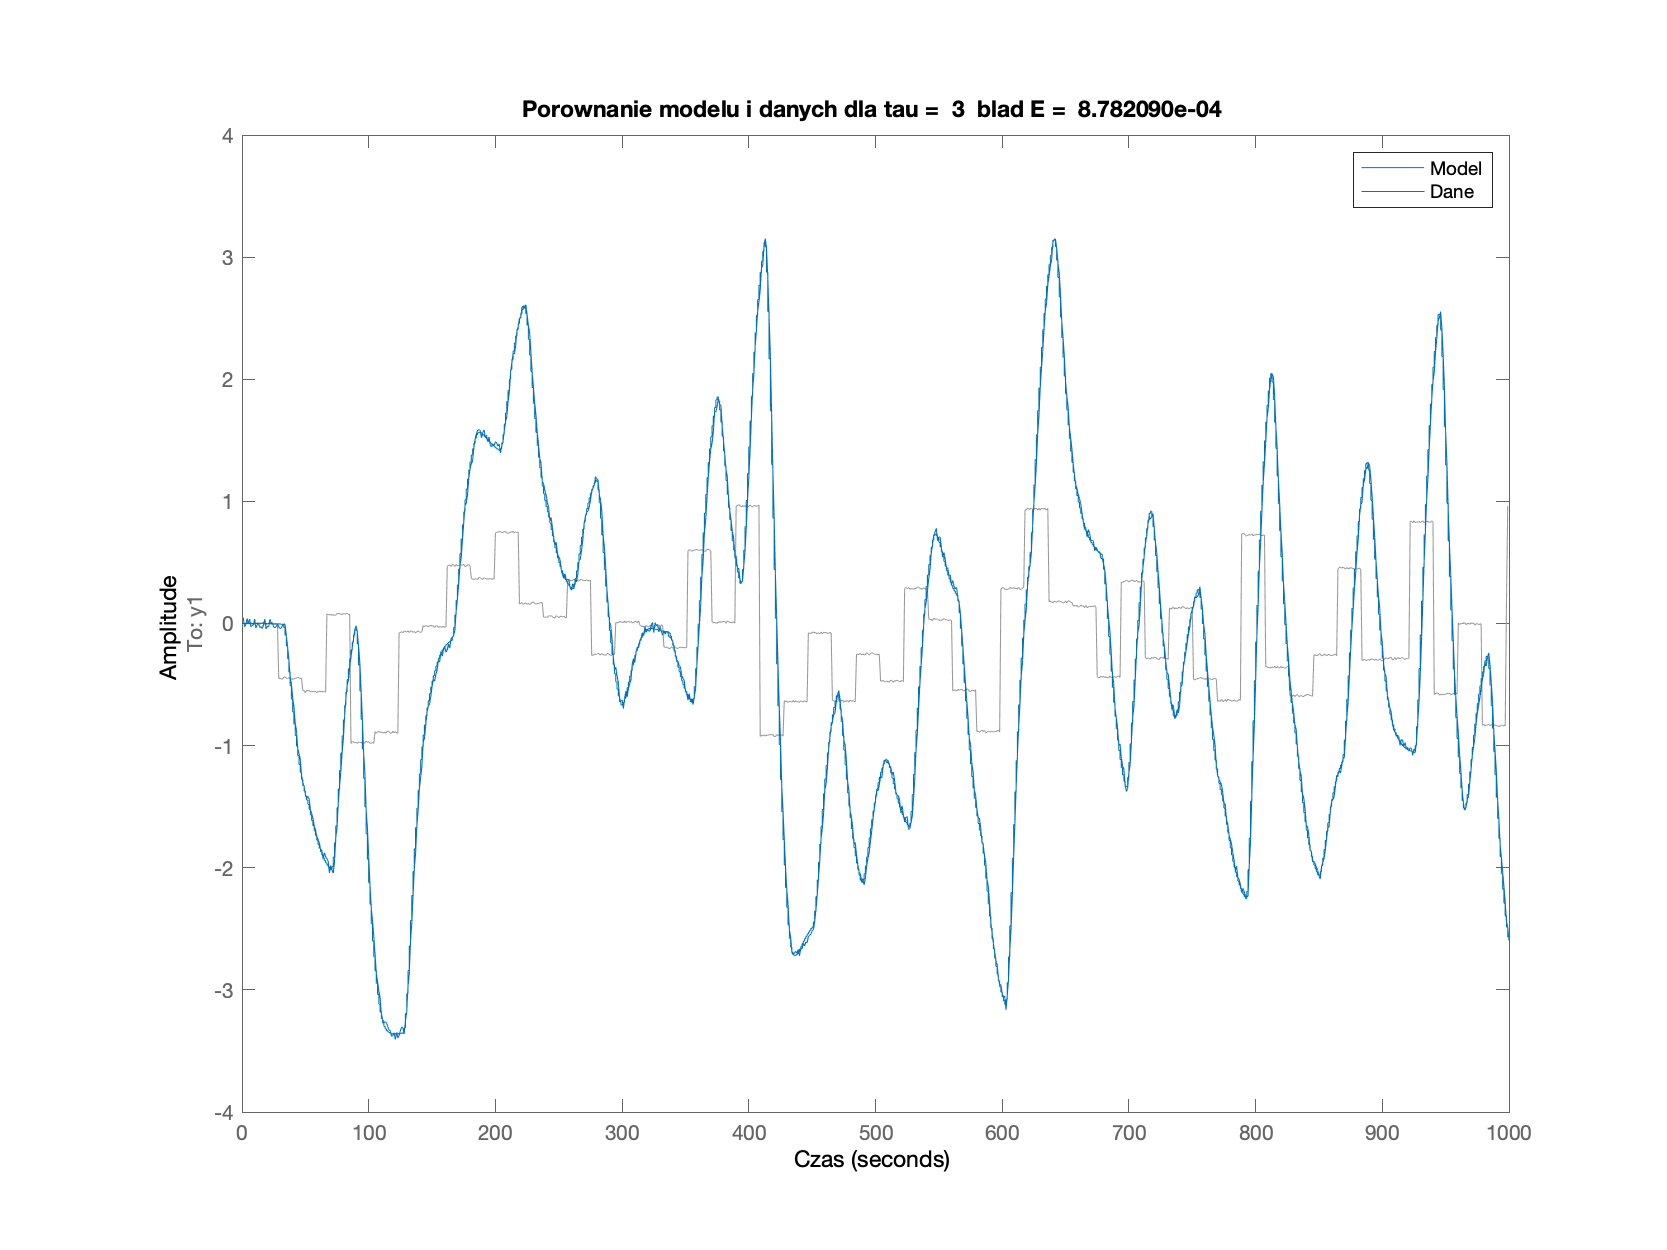
\includegraphics[width=\linewidth]{./ModelsP1/modelTau3.png}
\caption[Model dla \(\tau = 3\) ]
{Model dla \(\tau = 3\)}
\end{figure}

Obliczona transmitancja to \[G(z) = -\frac{0.0535\,z^{-4}+0.05131^{-5}}{1-1.664\,z^{-1}+0.692\,z^{-2}}\]
Błędy dla kolejnych wartości opóźnienia : 
\begin{table}[h]
\begin{tabular}{|l|l|l|l|}
\hline
\(\tau\) & Błąd & \(\tau\) & Błąd \\
\hline \hline
0 & 0.00439310239906314   & 1 & 0.00183921094764360  \\
2 & 0.00109013781103131   & 3 & 0.000878208985142877 \\
4 & 0.00127255618226417   & 5 & 0.00265973087538625  \\
6 & 0.00466320637124297   & 7 & 0.00657471083346129  \\
8 & 0.0144459616721526    & 9 & 0.0291933730835489   \\
10 & 0.0505076805408859    & 11 & 0.0815671234071185   \\
12 & 0.115793906377645     & 13 & 0.141062965735366    \\
14 & 0.192723451767430     & 15 & 0.224393357249063    \\
16 & 0.279145538665909     & 17 & 0.327832479282838    \\
18 & 0.266753410572330     & 19 & 0.526295935361537    \\
20 & 6.68422436659490    & X&X\\
\hline
\end{tabular}
\end{table}
\newpage
Jak widać błąd jest najmniejszy dla opóźnienia równego 3.
Ponieżej podaje przykładowe inne modele dla porównania.Można zauważyć że dla opóźnienia \(\tau = 3\) odwzorowanie jest najwierniejsze.\\*

\begin{figure*}[h]
\centering
        \begin{subfigure}[b]{0.475\textwidth}
			\centering
			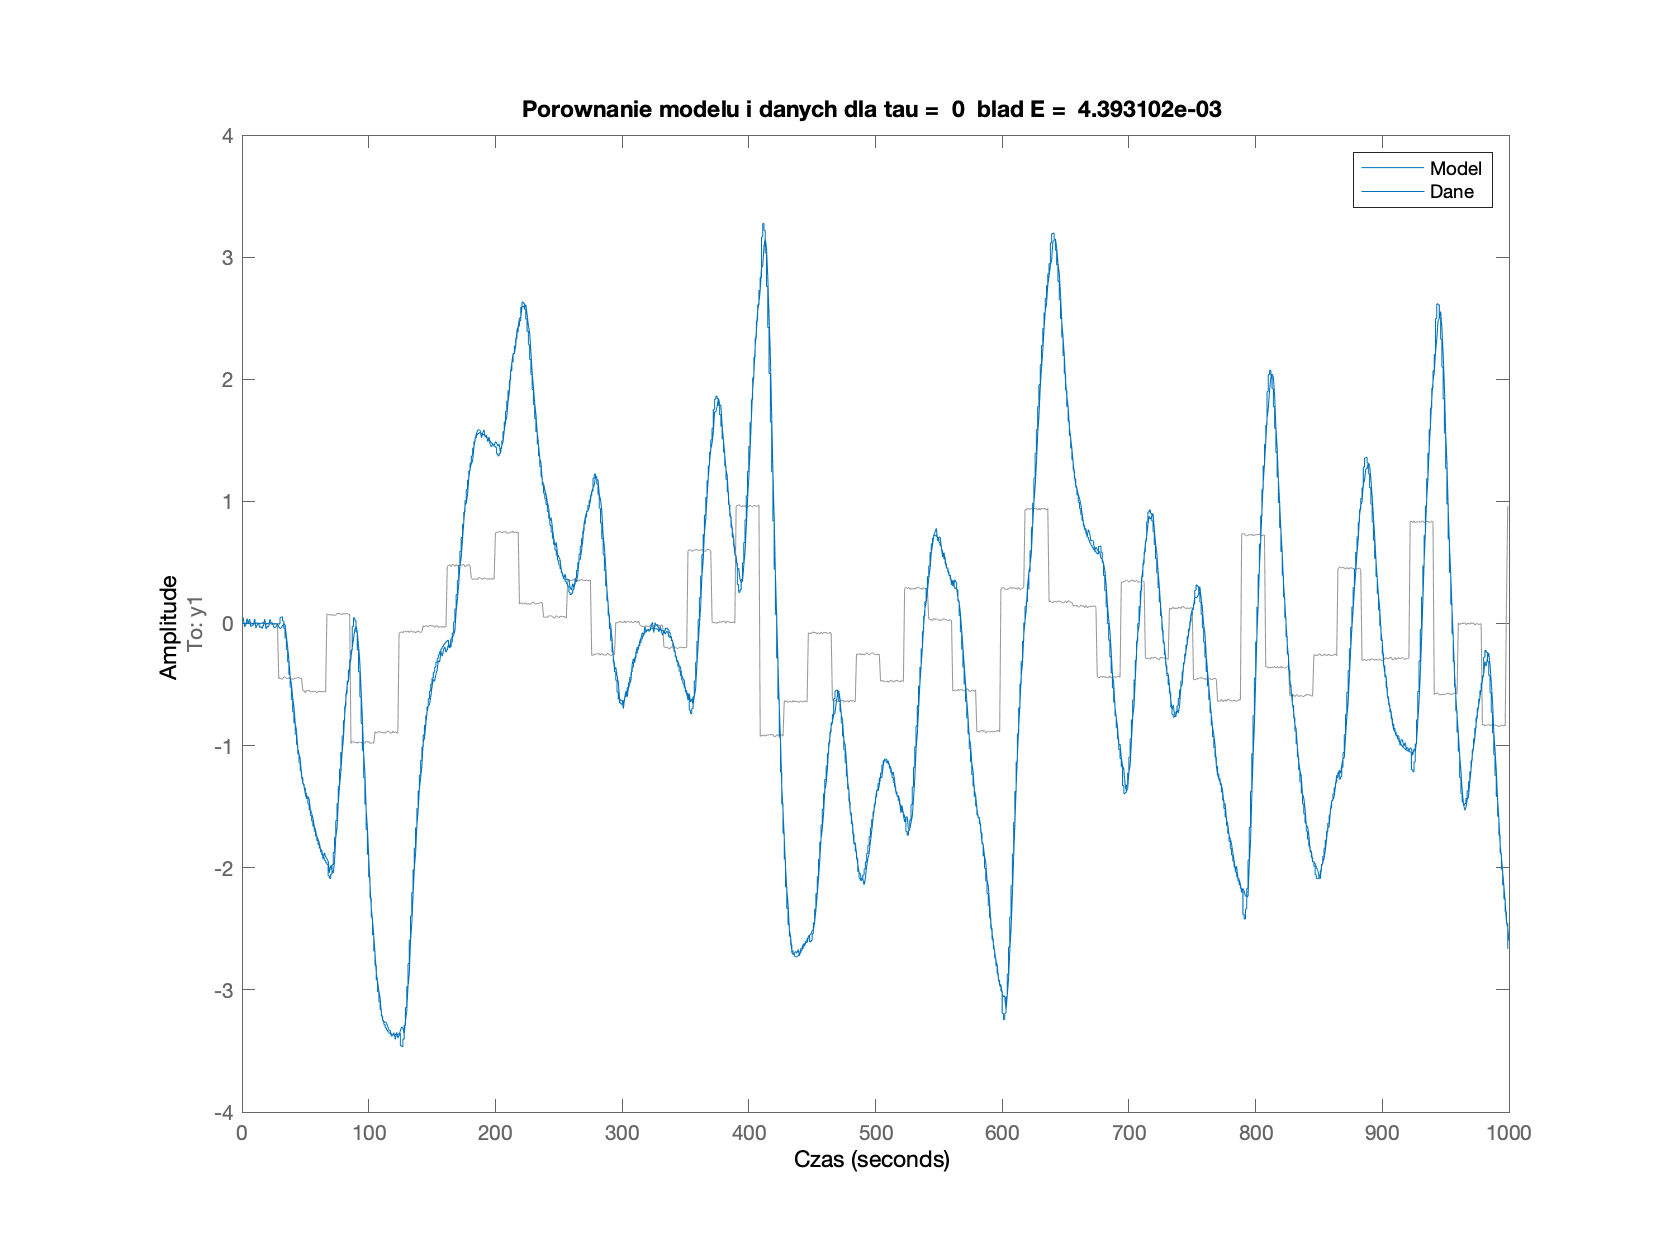
\includegraphics[width=\linewidth]{./ModelsP1/modelTau0.png}
			\caption[Model dla \(\tau = 0\) ]
			{Model dla \(\tau = 0\)}
		\end{subfigure}
		\hfill
        \begin{subfigure}[b]{0.475\textwidth}
			\centering
			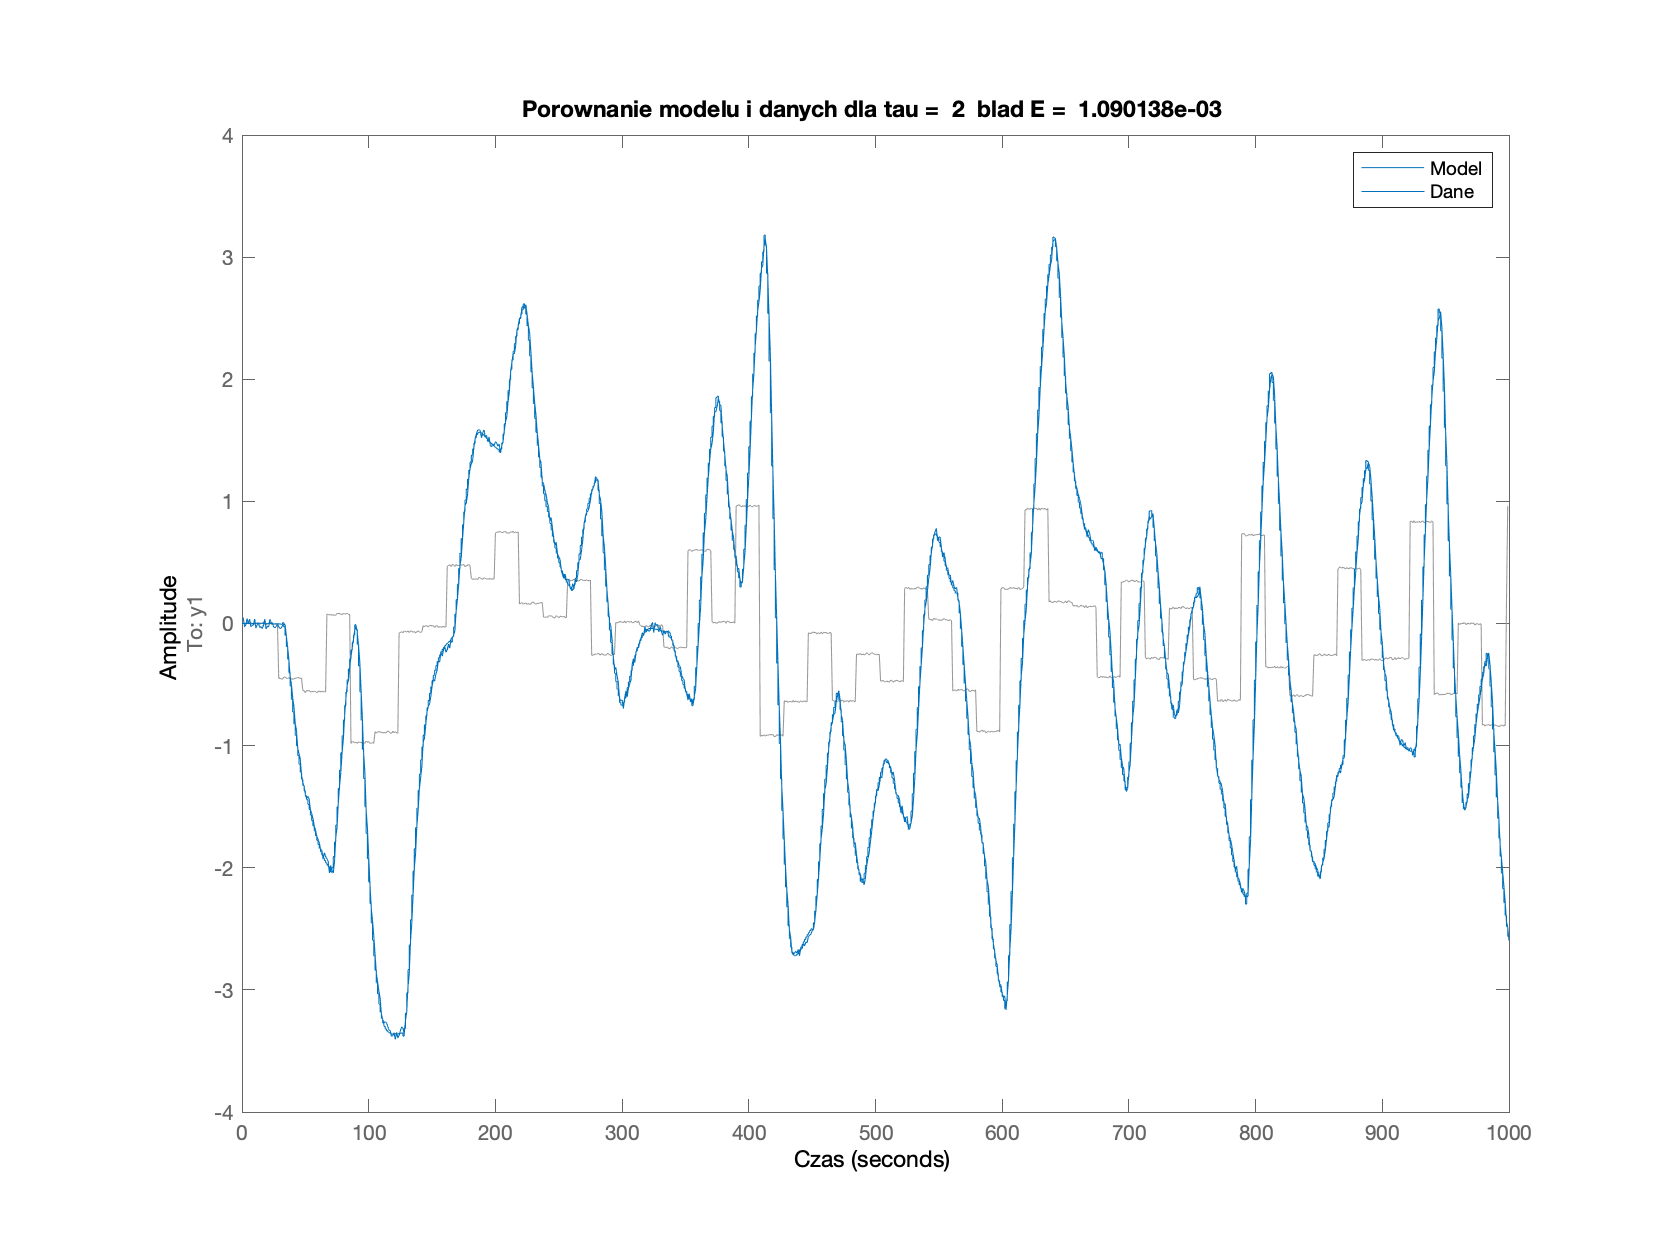
\includegraphics[width=\linewidth]{./ModelsP1/modelTau2.png}
			\caption[Model dla \(\tau = 2\) ]
			{Model dla \(\tau = 2\)}
		\end{subfigure}
        \vskip\baselineskip
        \begin{subfigure}[b]{0.475\textwidth}
			\centering
			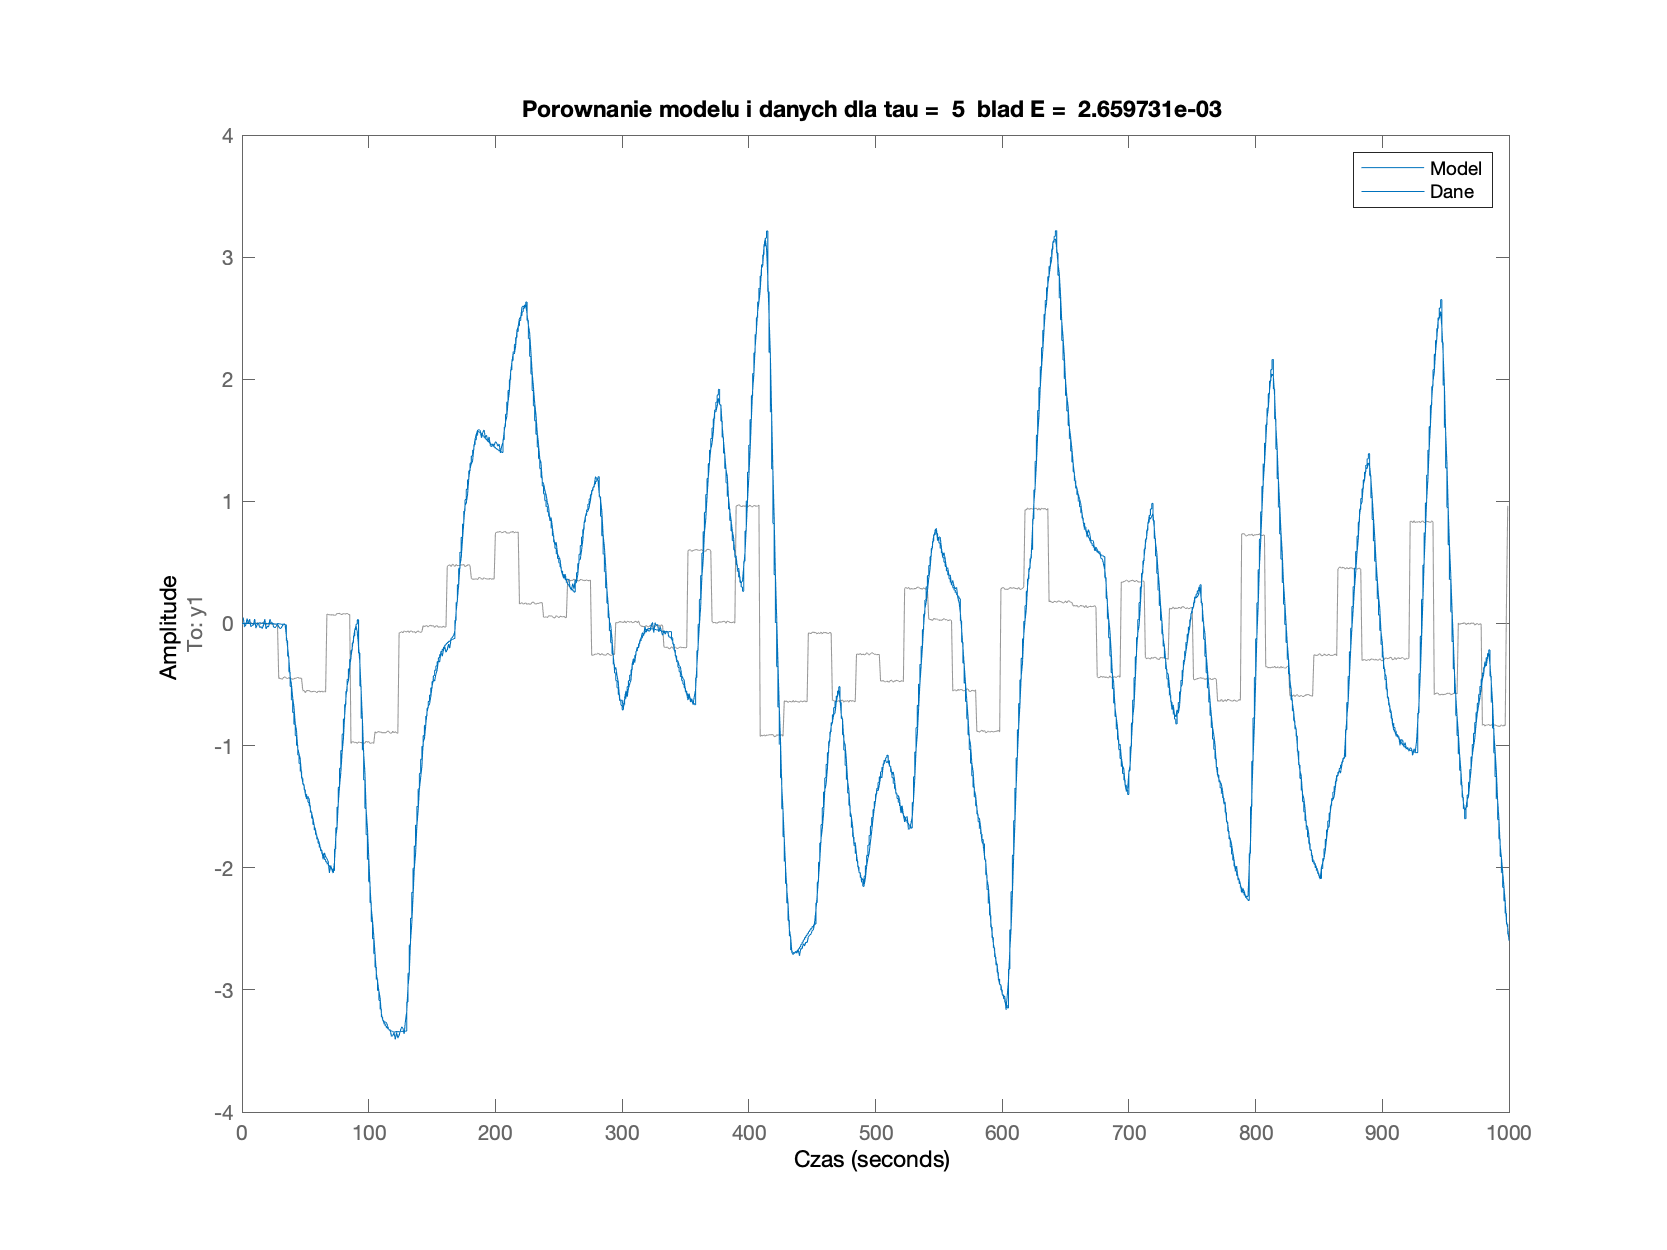
\includegraphics[width=\linewidth]{./ModelsP1/modelTau5.png}
			\caption[Model dla \(\tau = 5\) ]
			{Model dla \(\tau = 5\)}
		\end{subfigure}
        \quad
        \begin{subfigure}[b]{0.475\textwidth}
			\centering
			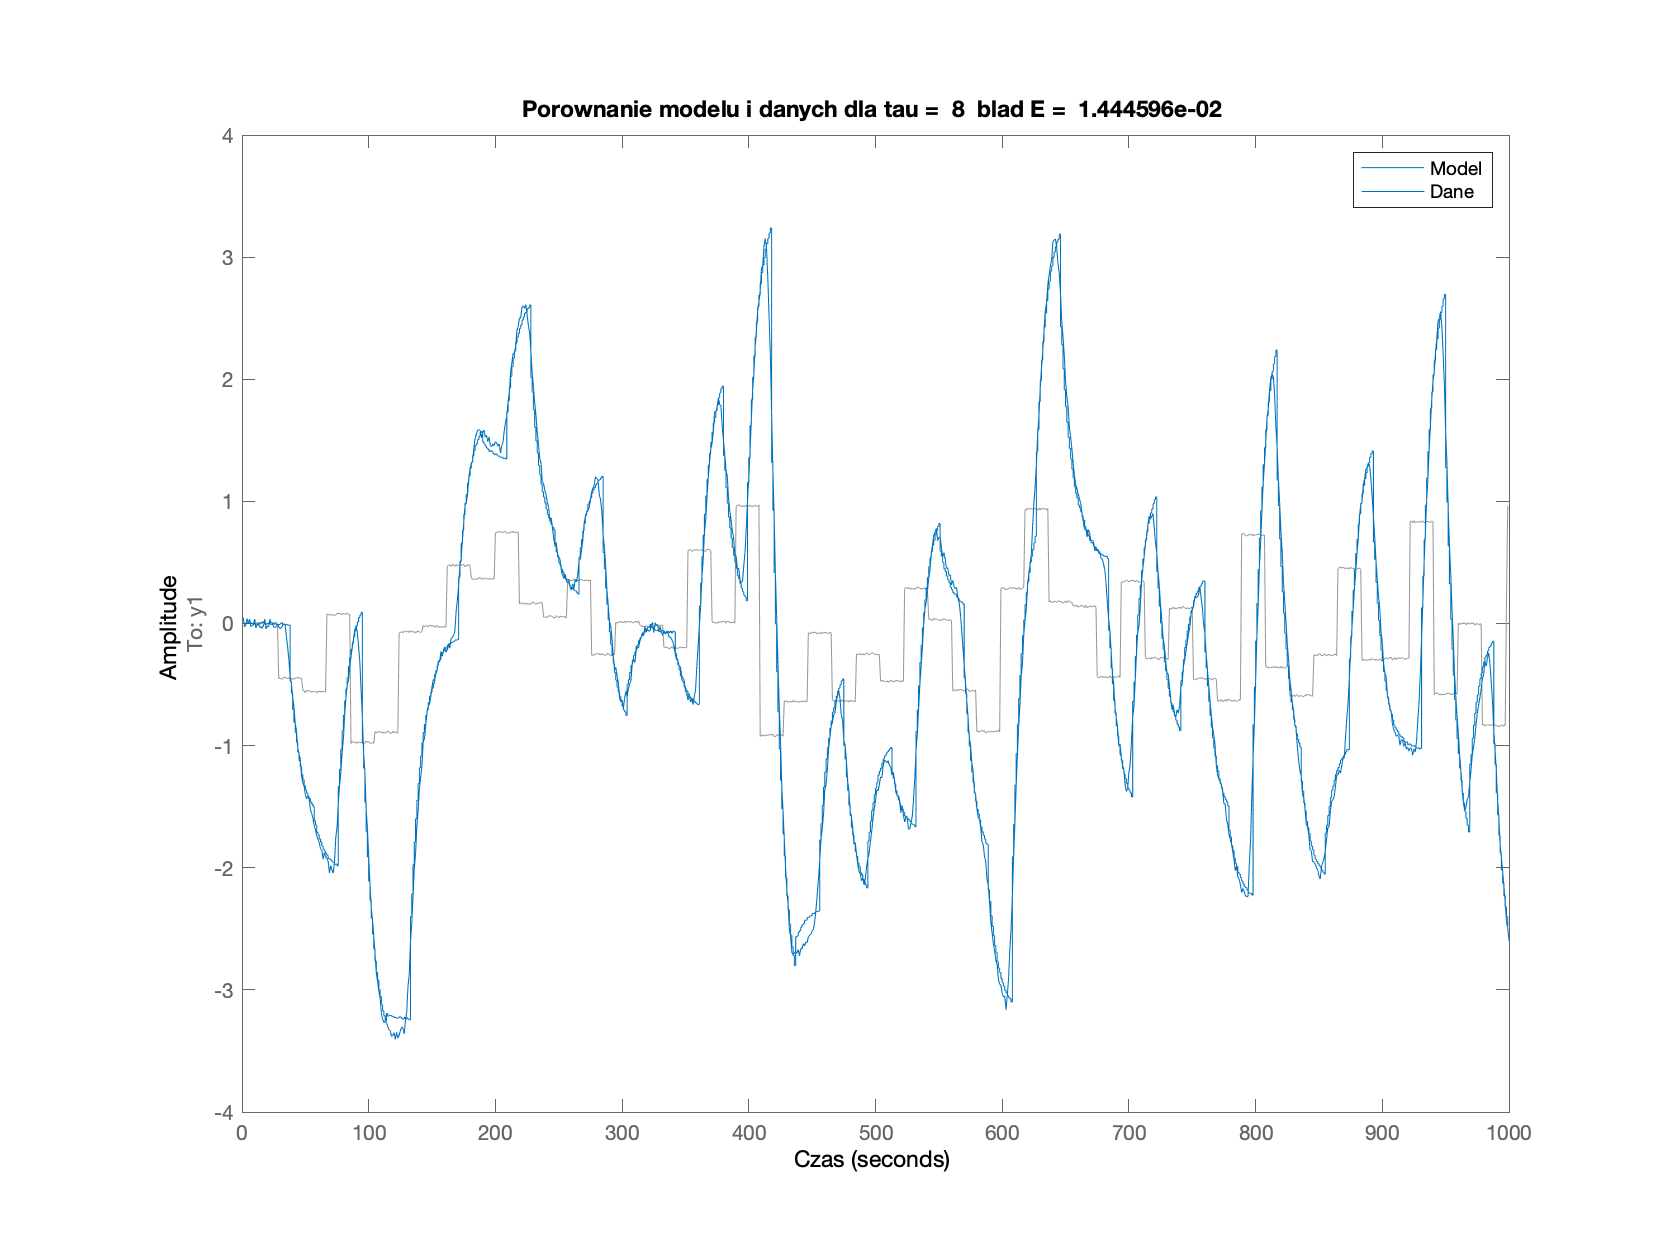
\includegraphics[width=\linewidth]{./ModelsP1/modelTau8.png}
			\caption[Model dla \(\tau = 8\) ]
			{Model dla \(\tau = 8\)}
		\end{subfigure}

\end{figure*}

\begin{figure*} 
\centering
        \begin{subfigure}[b]{0.475\textwidth}
			\centering
			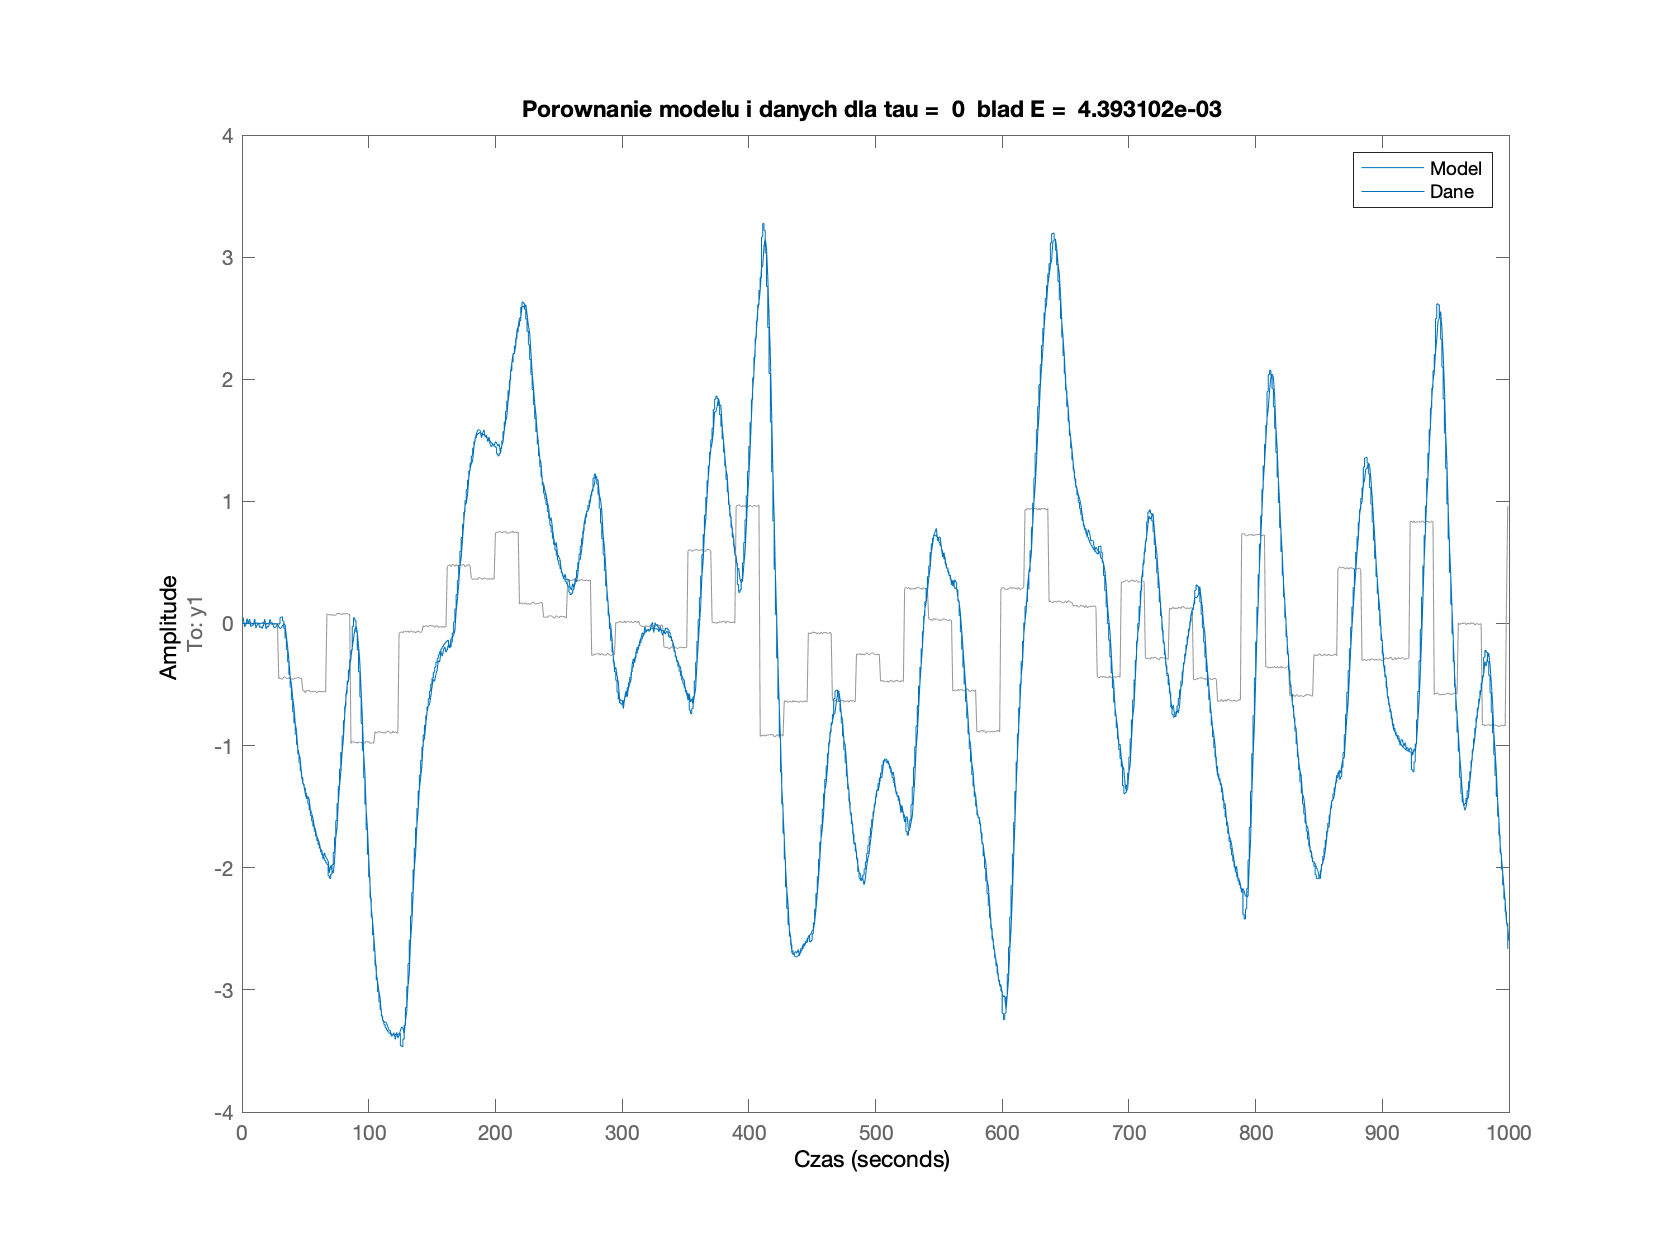
\includegraphics[width=\linewidth]{./ModelsP1/modelTau0.png}
			\caption[Model dla \(\tau = 10\) ]
			{Model dla \(\tau = 10\)}
		\end{subfigure}
		\hfill
        \begin{subfigure}[b]{0.475\textwidth}
			\centering
			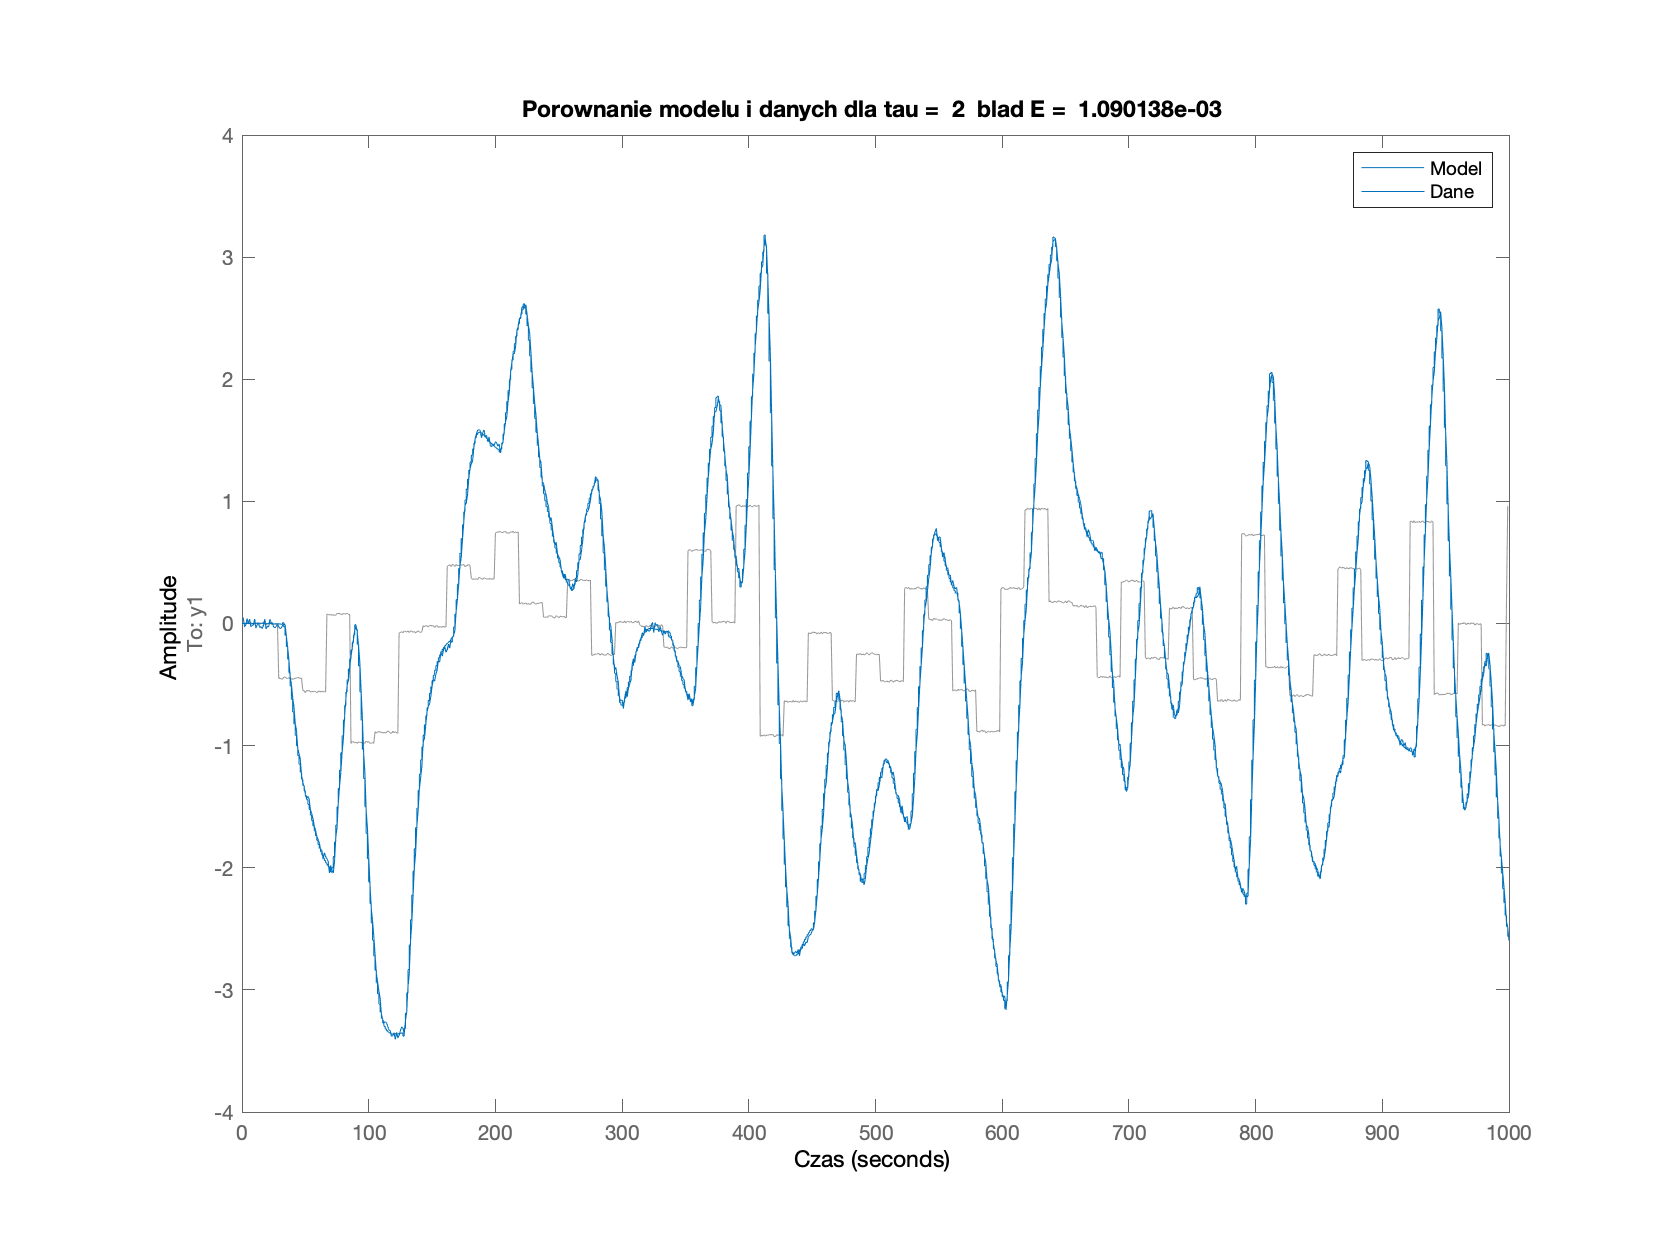
\includegraphics[width=\linewidth]{./ModelsP1/modelTau2.png}
			\caption[Model dla \(\tau = 12\) ]
			{Model dla \(\tau = 12\)}
		\end{subfigure}
        \vskip\baselineskip
        \begin{subfigure}[b]{0.475\textwidth}
			\centering
			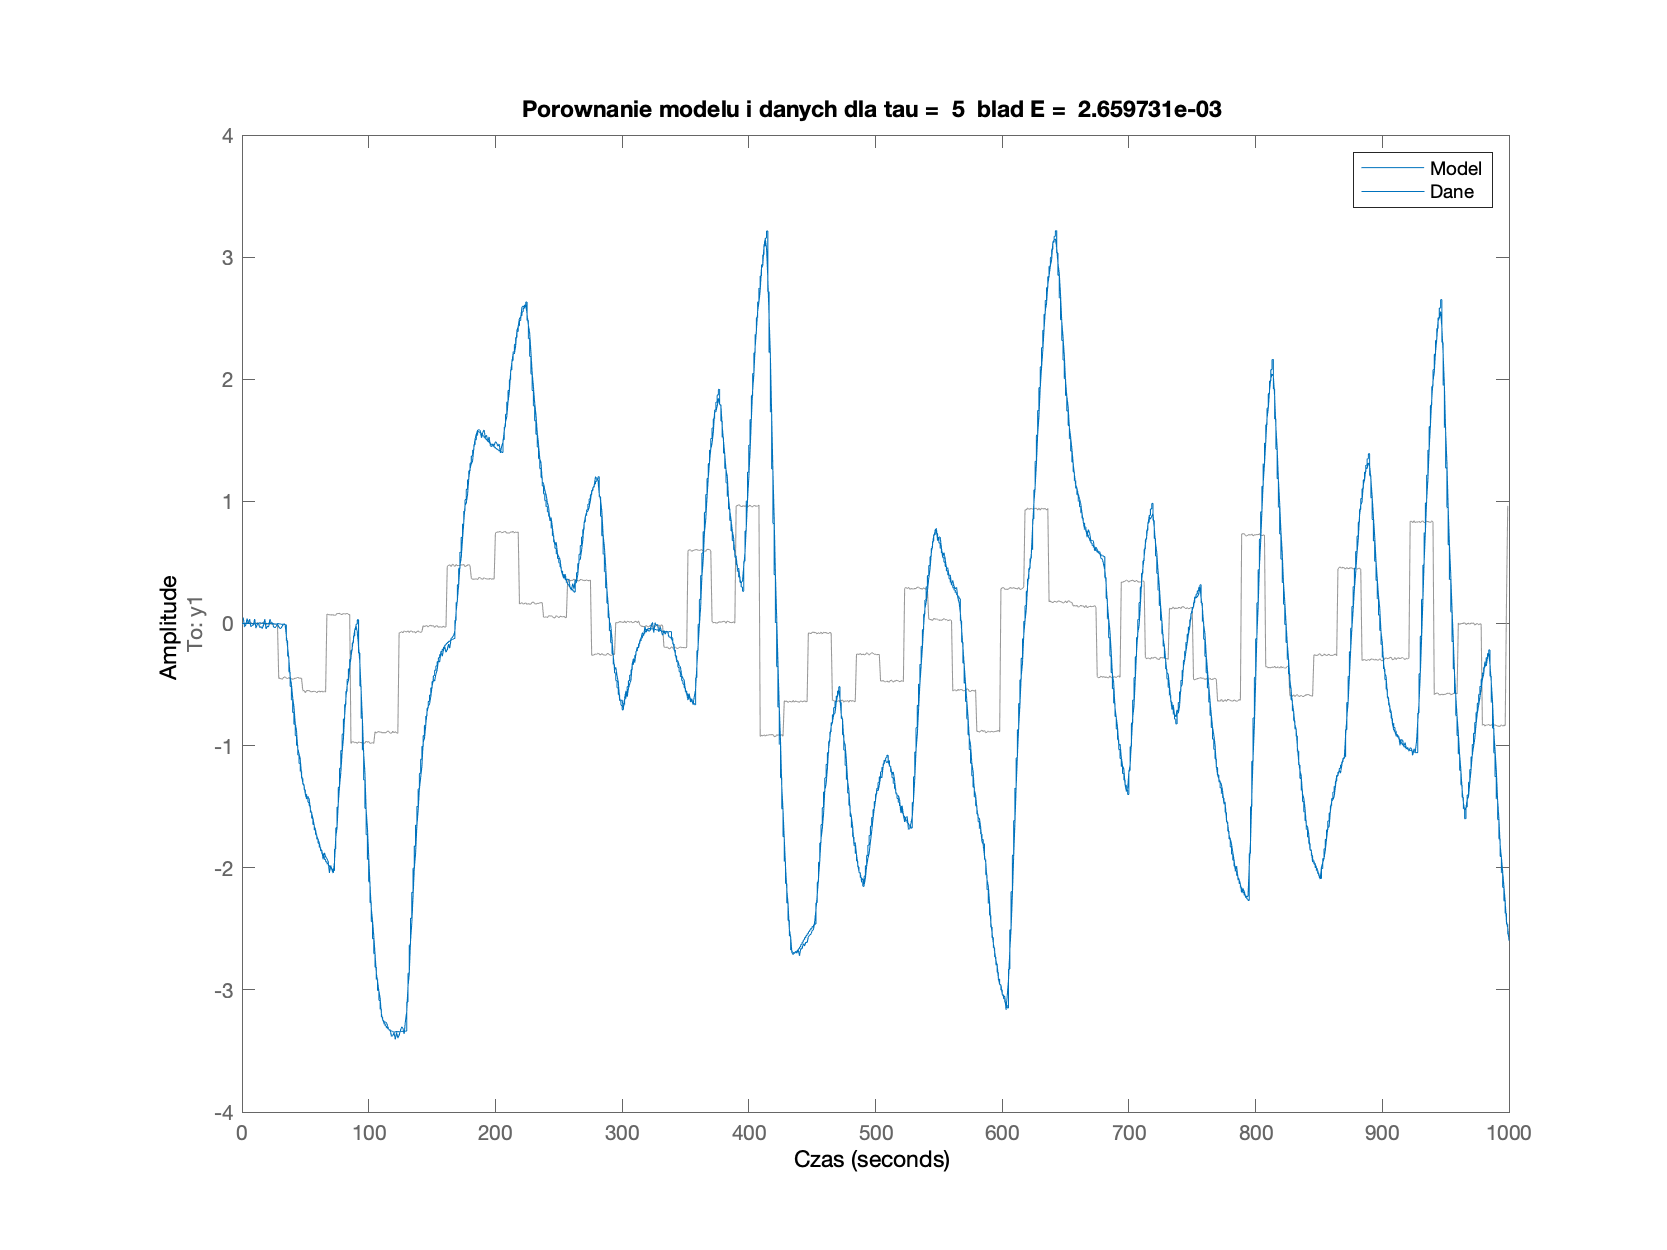
\includegraphics[width=\linewidth]{./ModelsP1/modelTau5.png}
			\caption[Model dla \(\tau =15\) ]
			{Model dla \(\tau = 15\)}
		\end{subfigure}
        \quad
        \begin{subfigure}[b]{0.475\textwidth}
			\centering
			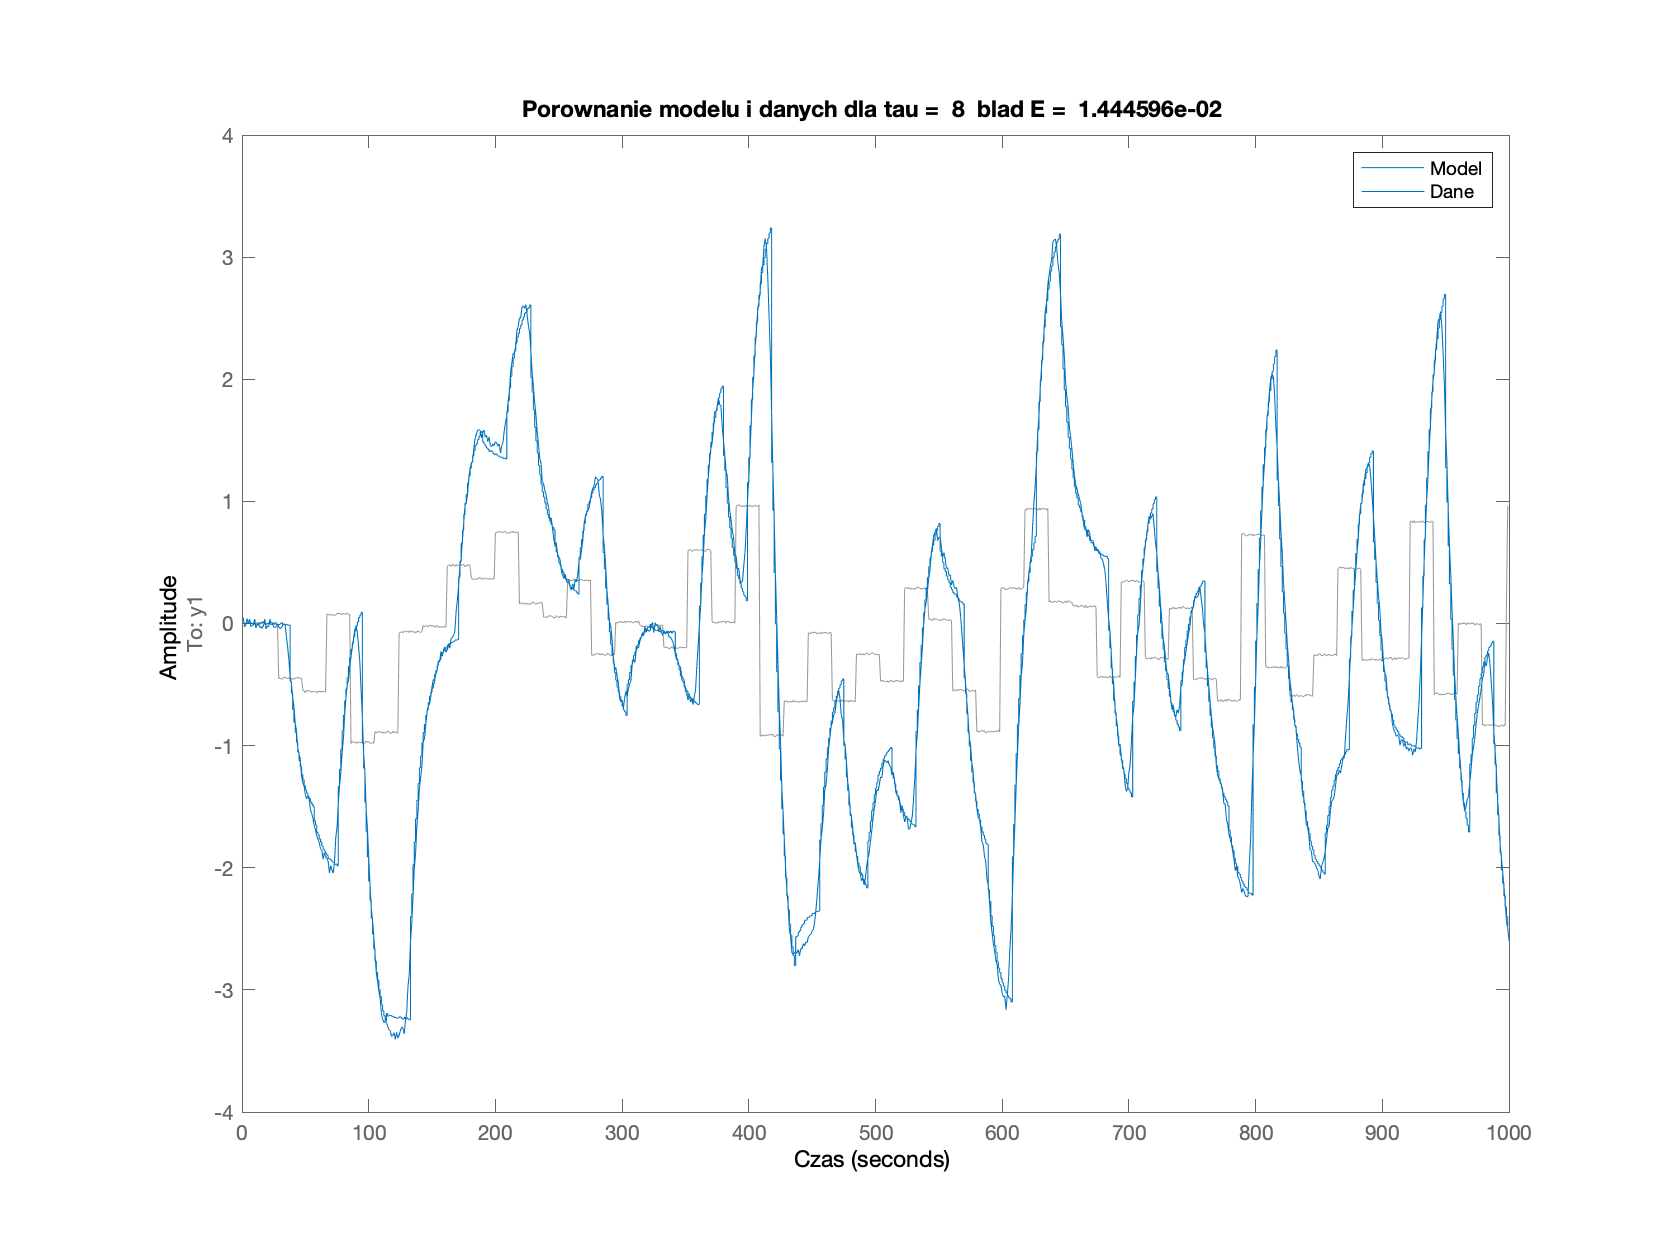
\includegraphics[width=\linewidth]{./ModelsP1/modelTau8.png}
			\caption[Model dla \(\tau = 20\) ]
			{Model dla \(\tau = 20\)}
		\end{subfigure}

\end{figure*}

\newpage
\begin{itemize}
\item Trasmitancja dla \(\tau = 0 \)
\[G(z) = -\frac{-0.1237\,z^{-1}+0.202^{-2}}{1-1.732\,z^{-1}+0.753\,z^{-2}}\]
\item Trasmitancja dla \(\tau =  2\)
\[G(z) = -\frac{-0.03262\,z^{-3}+0.132^{-4}}{1-1.678\,z^{-1}+0.7041\,z^{-2}}\]
\item Trasmitancja dla \(\tau =  5\)
\[G(z) = -\frac{0.2905\,z^{-6}-0.2136^{-7}}{1-1.725\,z^{-1}+0.7455\,z^{-2}}\]
\item Trasmitancja dla \(\tau =  8\)
\[G(z) = -\frac{1.03\,z^{-9}-0.5651^{-10}}{1-1.0.7708\,z^{-1}-0.1014\,z^{-2}}\]
\item Trasmitancja dla \(\tau =  10\)
\[G(z) = -\frac{1.463\,z^{-11}-1.075^{-12}}{1-0.9145\,z^{-1}+0.026\,z^{-2}}\]
\item Trasmitancja dla \(\tau =  12\)
\[G(z) = -\frac{1.741\,z^{-13}-1.463^{-14}}{1-1.048\,z^{-1}+0.1325\,z^{-2}}\]
\item Trasmitancja dla \(\tau =  15\)
\[G(z) = -\frac{2.085\,z^{-16}-1.941^{-17}}{1-1.078\,z^{-1}+0.1273\,z^{-2}}\]
\item Trasmitancja dla \(\tau =  20\)
\[G(z) = -\frac{2.306\,z^{-21}-2.116^{-22}}{1-0.8561\,z^{-1}-0.0563\,z^{-2}}\]
\end{itemize}
\newpage

Kod użyty do policzenia punktu 1go:
 \lstinputlisting{P1.m} 
\newpage
\item
Wzmocnienie statyczne : K = 3,7432 \\
Odpowiedź skokowa :
\begin{figure}[h]
\centering
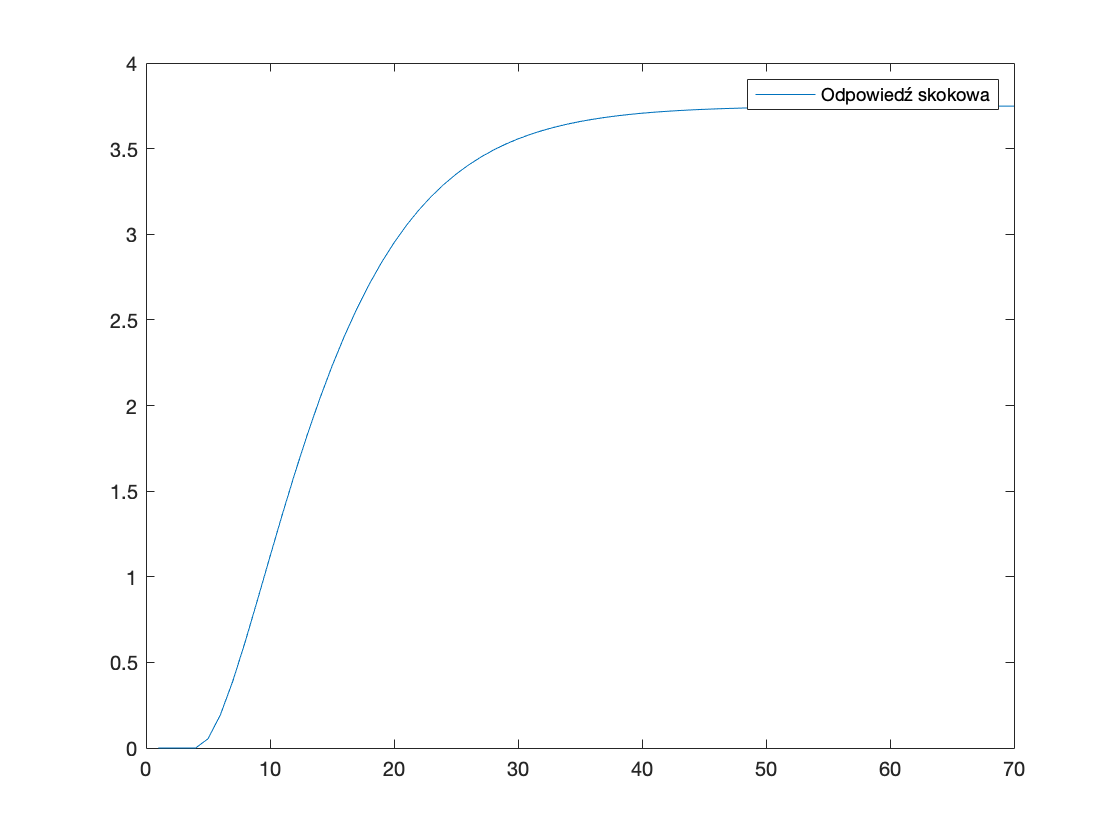
\includegraphics[width=\linewidth]{./OdpSkokowa.png}
\caption[Odpowiedź skokowa dla \(\tau = 3\) ]
{Odpowiedź skokowa dla \(\tau = 3\) }
\end{figure}
\\
Oraz w formie tabeli : \\
\newpage
 \begin{table}[h]
\begin{tabular}{|l|l|l|l|l|l|}
\hline
I & 1            & 2            & 3           & 4            & 5             \\
\hline
S & 0            & 0            & 0           & 0            & 0.05350337749 \\
\hline
\hline
I & 6            & 7            & 8           & 9            & 10            \\
\hline
S & 0.1938495617 & 0.3903675229 & 0.620261978 & 0.8668251224 & 1.118028917   \\
\hline
\hline
I & 11           & 12           & 13          & 14           & 15            \\
\hline
S & 1.365420087  & 1.60325549   & 1.827828011 & 2.036943139  & 2.22951446    \\
\hline
\hline
I & 16           & 17           & 18          & 19           & 20            \\
\hline
S & 2.405252755  & 2.564428553  & 2.707692175 & 2.835938574  & 2.950206968   \\
\hline
\hline
I & 21           & 22           & 23          & 24           & 25            \\
\hline
S & 3.051607351  & 3.141267655  & 3.220296689 & 3.289759025  & 3.350658852   \\
\hline
\hline
I & 26           & 27           & 28          & 29           & 30            \\
\hline
S & 3.403930501  & 3.450433829  & 3.49095312  & 3.526198425  & 3.556808576   \\
\hline
\hline
I & 31           & 32           & 33          & 34           & 35            \\
\hline
S & 3.583355254  & 3.606347689  & 3.626237655 & 3.643424532  & 3.658260277   \\
\hline
\hline
I & 36           & 37           & 38          & 39           & 40            \\
\hline
S & 3.671054189  & 3.682077398  & 3.69156704  & 3.699730096  & 3.706746891   \\
\hline
\hline
I & 41           & 42           & 43          & 44           & 45            \\
\hline
S & 3.712774264  & 3.717948414  & 3.722387449 & 3.726193656  & 3.729455513   \\
\hline
\hline
I & 46           & 47           & 48          & 49           & 50            \\
\hline
S & 3.73224947   & 3.734641511  & 3.736688539 & 3.738439577  & 3.739936825   \\
\hline
\hline
I & 51           & 52           & 53          & 54           & 55            \\
\hline
S & 3.741216583  & 3.742310053  & 3.743244033 & 3.744041531  & 3.744722282   \\
\hline
\hline
I & 56           & 57           & 58          & 59           & 60            \\
\hline
S & 3.745303209  & 3.745798813  & 3.746221515 & 3.746581948  & 3.746889213   \\
\hline
\hline
I & 61           & 62           & 63          & 64           & 65            \\
\hline
S & 3.747151093  & 3.747374245  & 3.747564356 & 3.747726286  & 3.747864188   \\
\hline
\hline
I & 66           & 67           & 68          & 69           & 70            \\
\hline
S & 3.747981606  & 3.748081566  & 3.748166649 & 3.748239059  & 3.748300673  \\
\hline

\end{tabular}
\end{table} 
Kod użyty do policzenia punktu 2go:
 \lstinputlisting{P2.m} 
\newpage
\item Algorytm PID - \(K_{kr} = 1.36 , T_{kr} = 20 \)\\
Oscylacje krytyczne metodą Zieglera-Nicholsa:
\begin{figure} [h]
\centering
 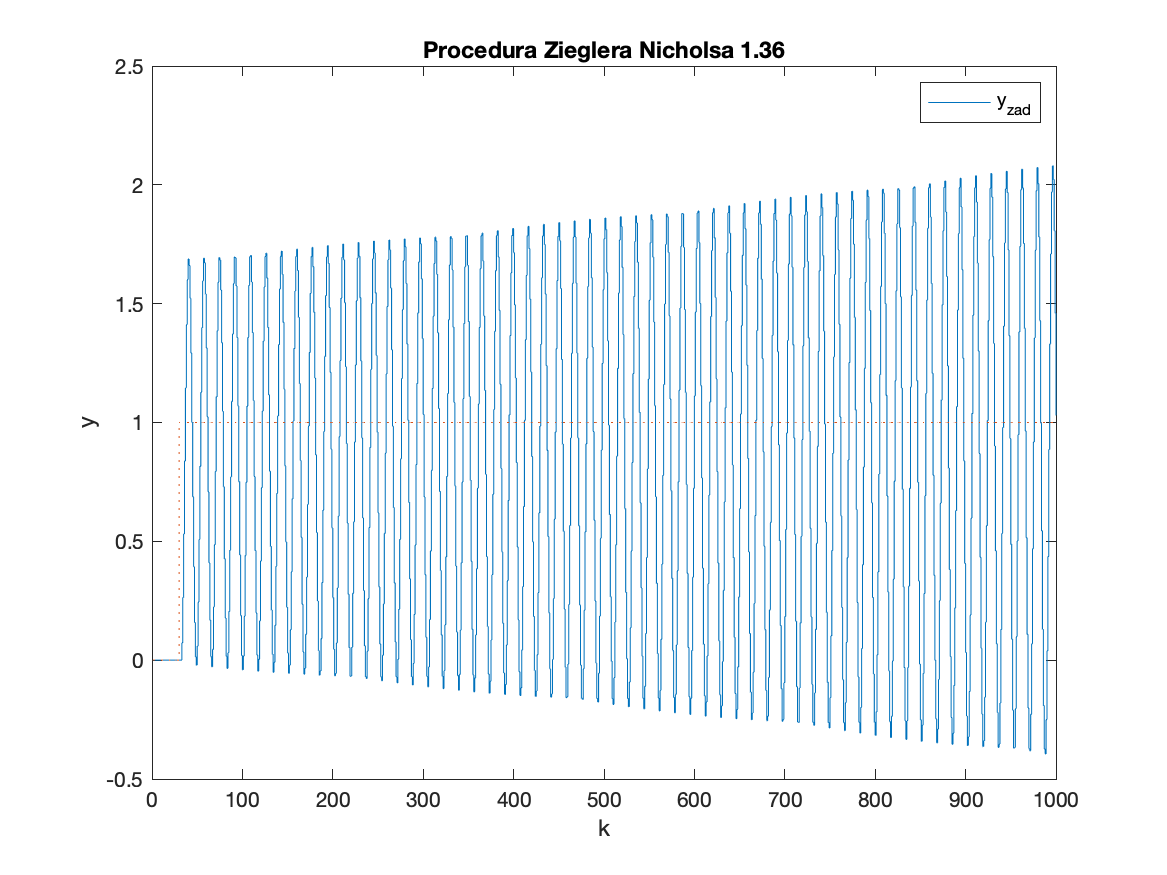
\includegraphics[width=\linewidth]{./ModelsP3/ZN/P2_K136png.png} 
\caption[Metoda Zieglera-Nicholsa]
{Metoda Zieglera-Nicholsa}
\end{figure}
\\
Wyznaczenie wzmocnienia krytycznego metodą Zieglera - Nicholsa : \\*
 \lstinputlisting{P3_ZN.m} 
Wykres dla algorytmu PID : 
\begin{figure}[h]
\centering
 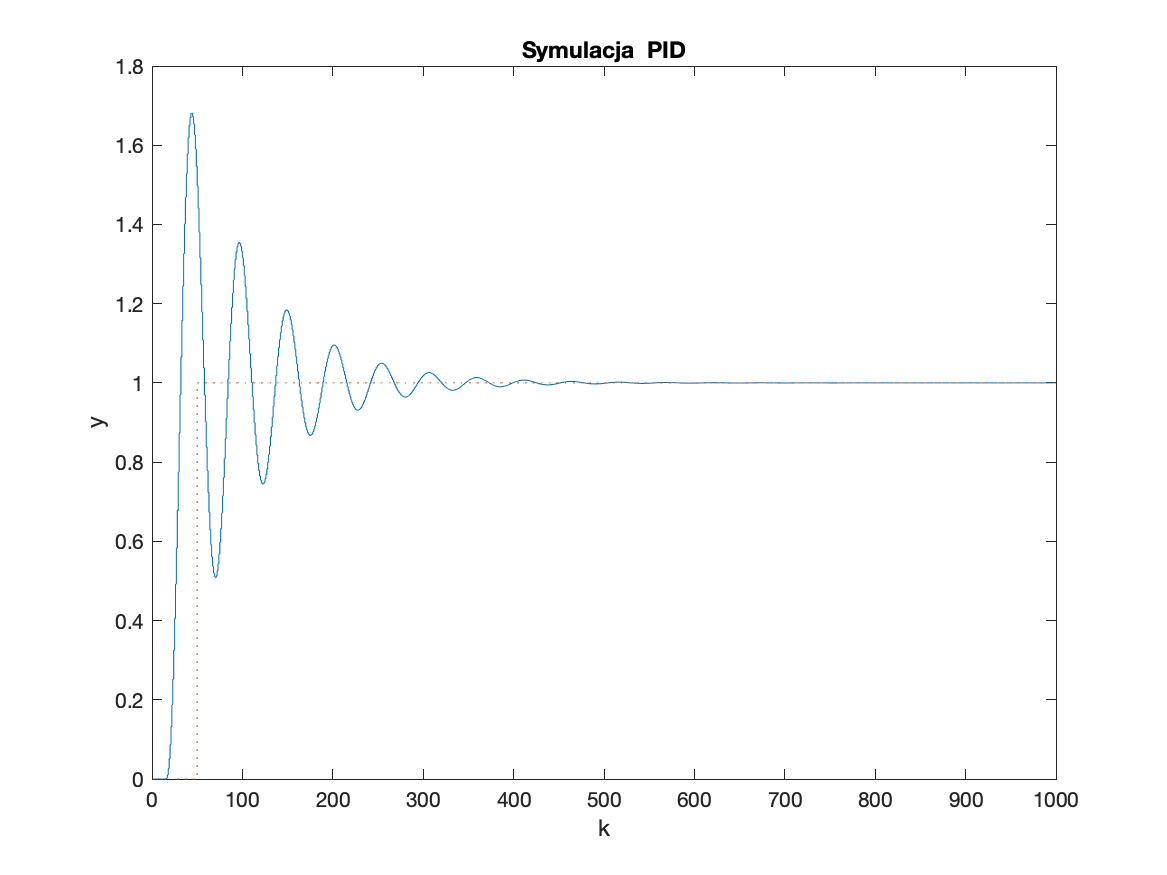
\includegraphics[width=\linewidth]{./ModelsP3/PID/P4-2_r1_47532r2_-86292r3_39168.png} 
\caption[Algorytm PID]
{Algorytm PID}
\end{figure}

Symulacja algorytmu PID : \\*
 \lstinputlisting{P3.m} 
\newpage
\item
Wyznaczanie parametrów DMC \\
Wyznaczone parametry :   D = 50, N = 15, Nu = 2, \(\lambda = 3 \)\\
\begin{figure} [h]
\centering
 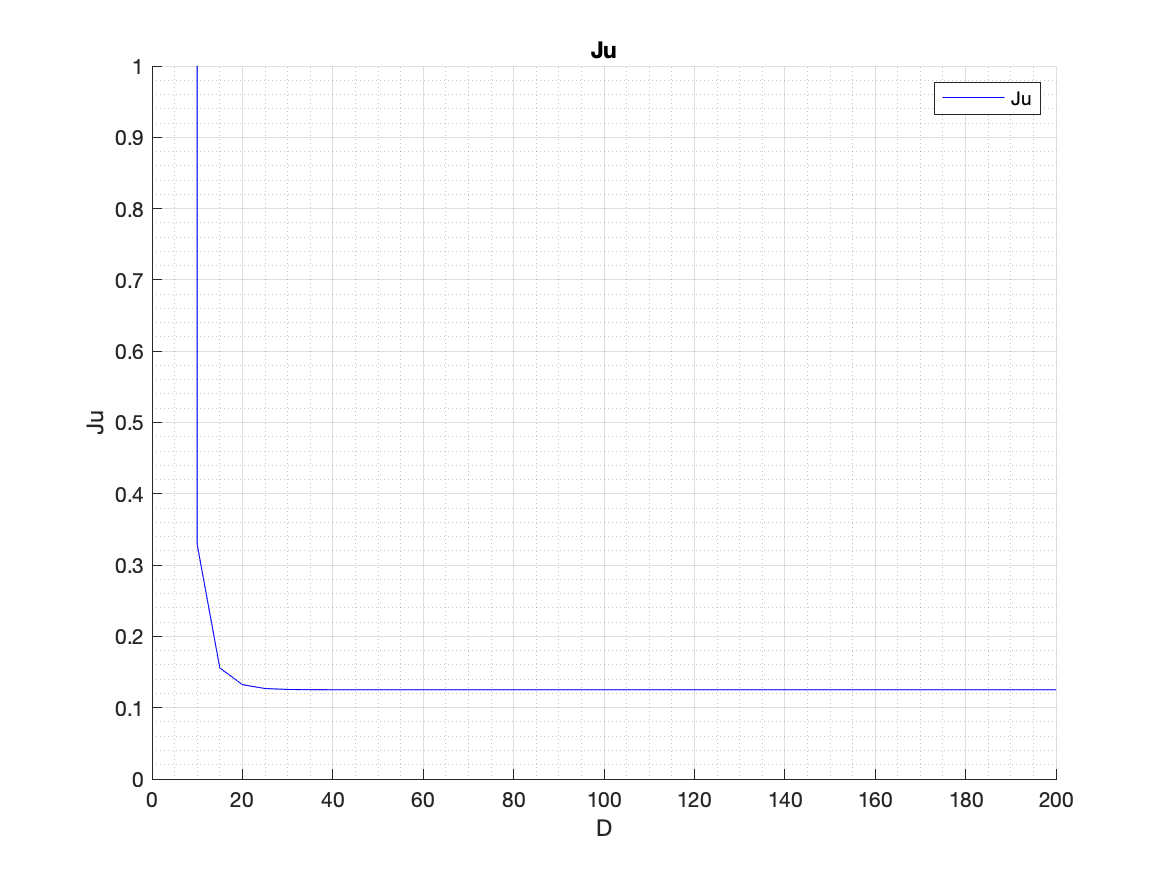
\includegraphics[width=\linewidth]{./ModelsP4_J/JuD.png} 
 \caption[Wyznaczone parametry Ju dla różnych wartości D]
{Wyznaczone parametry Ju dla różnych wartości D}
 \end{figure}
 
 \begin{figure} [h]
\centering
 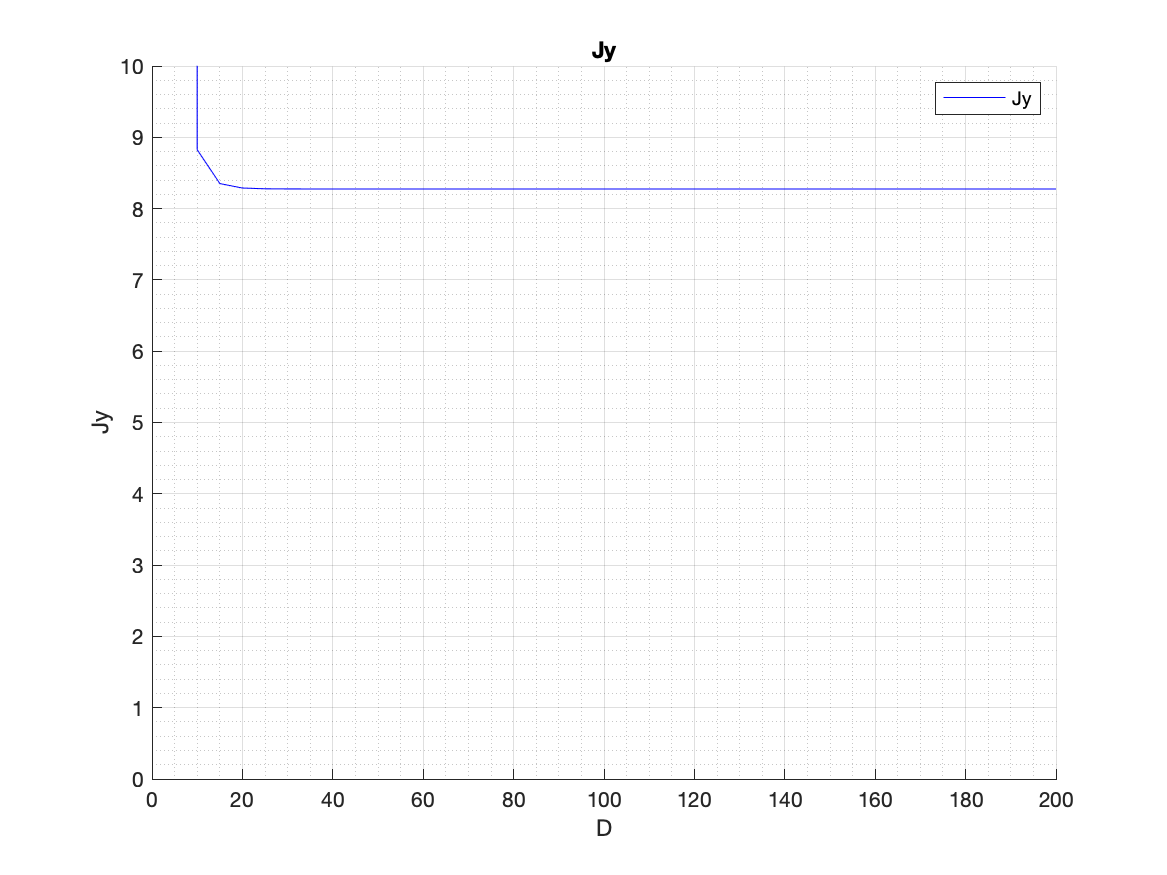
\includegraphics[width=\linewidth]{./ModelsP4_J/JyD.png} 
 \caption[Wyznaczone parametry Jy dla różnych wartości D]
{Wyznaczone parametry Jy dla różnych wartości D}
 \end{figure}
 
\begin{figure} [H]
\centering
 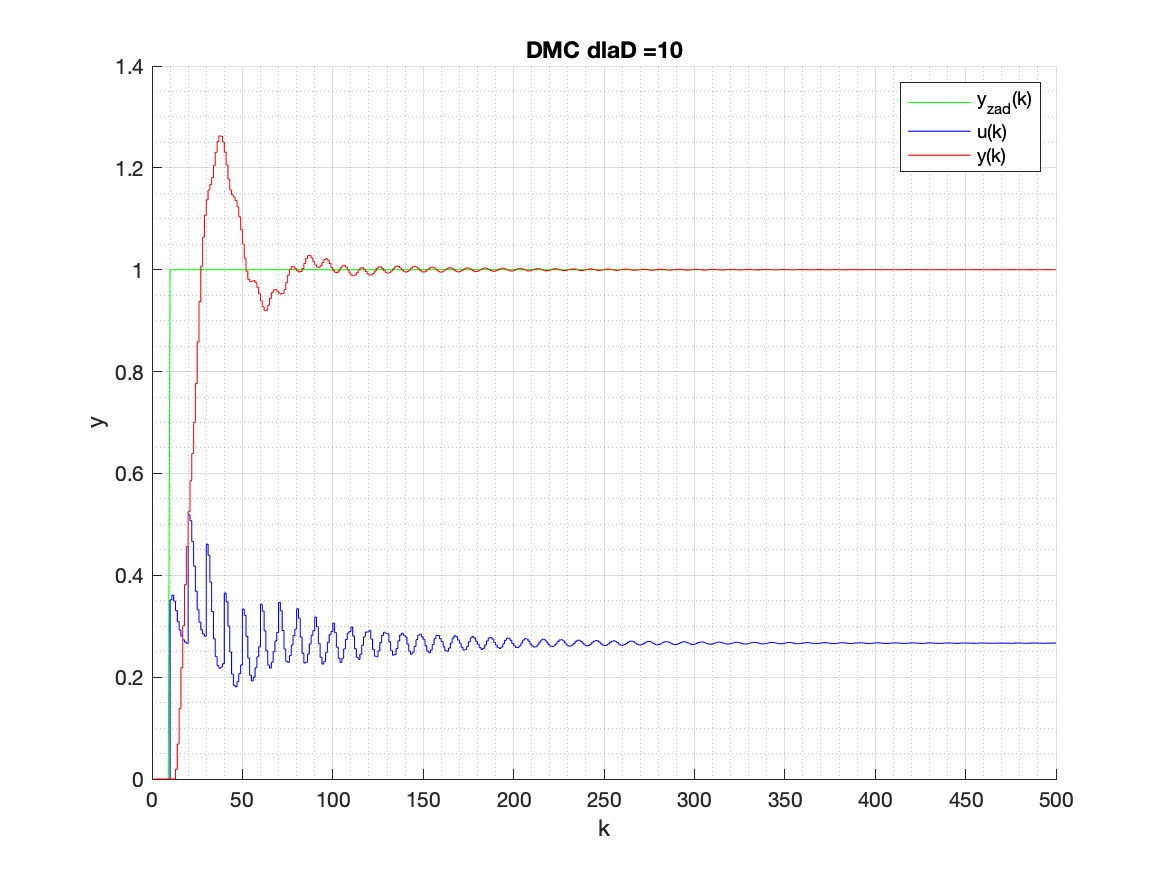
\includegraphics[width=\linewidth]{./ModelsP4_D/P4_DMC_D_10_png.png} 
 \caption[Różne wartości D - przebiegi DMC]
{Różne wartości D - przebiegi DMC}
 \end{figure}
 
 \begin{figure} [h]
\centering
 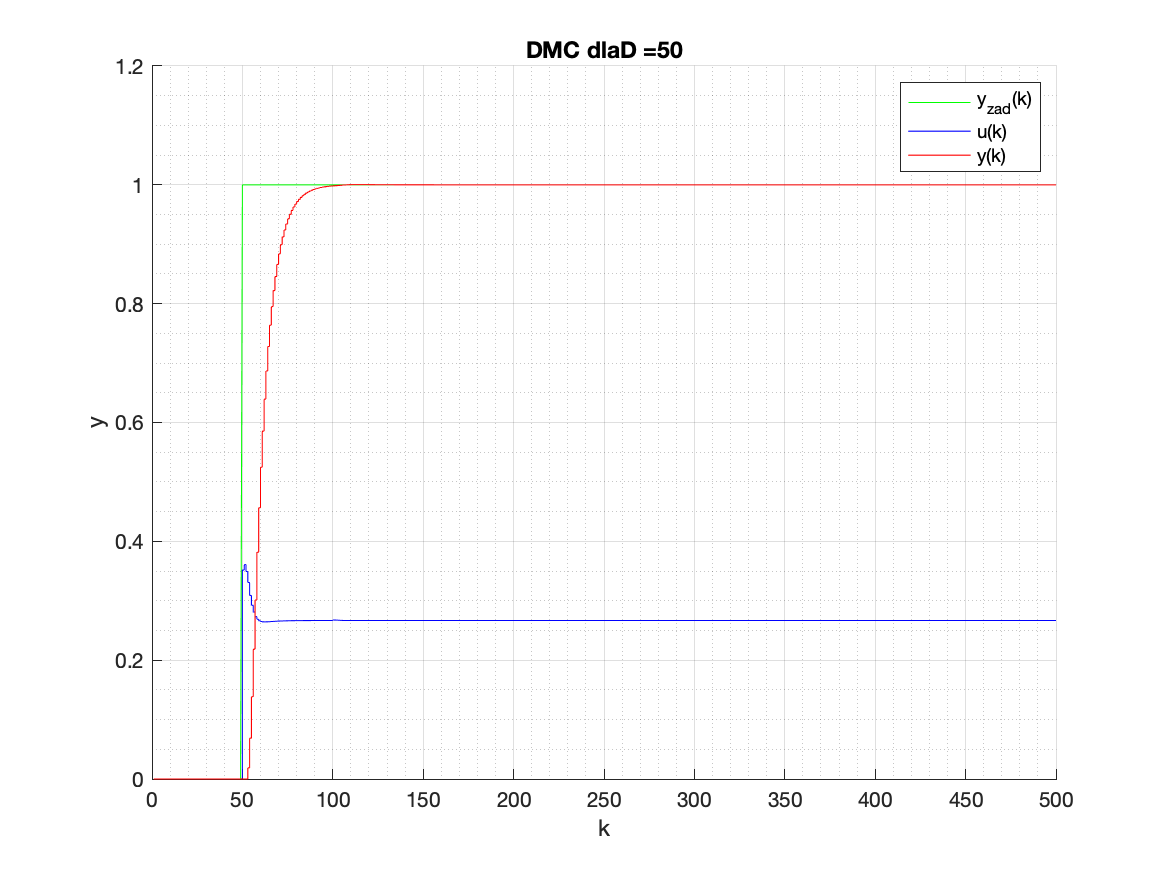
\includegraphics[width=\linewidth]{./ModelsP4_D/P4_DMC_D_50_png.png} 
 \caption[Różne wartości D - przebiegi DMC]
{Różne wartości D - przebiegi DMC}
 \end{figure}
 
 \begin{figure} [H]
\centering
  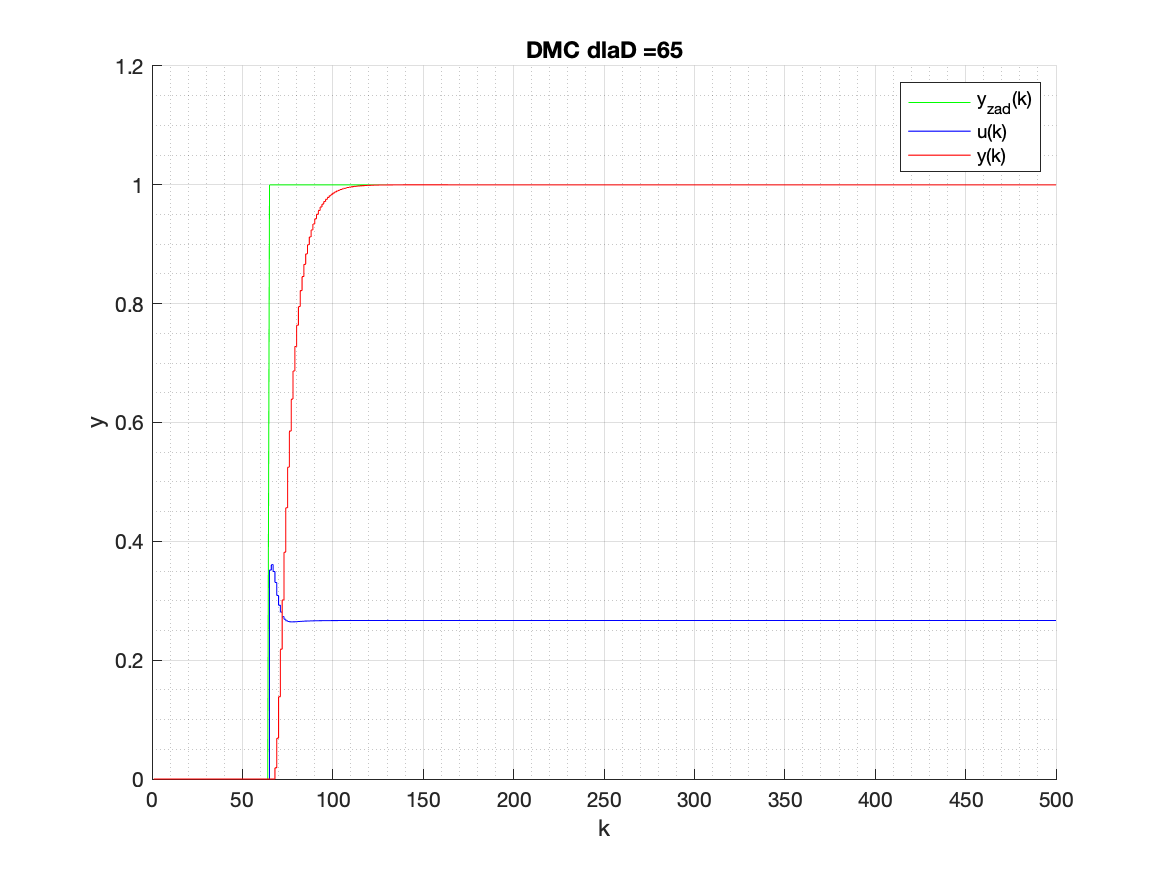
\includegraphics[width=\linewidth]{./ModelsP4_D/P4_DMC_D_65_png.png} 
 \caption[Różne wartości D - przebiegi DMC]
{Różne wartości D - przebiegi DMC}
 \end{figure}
 
 \begin{figure} [h]
\centering
 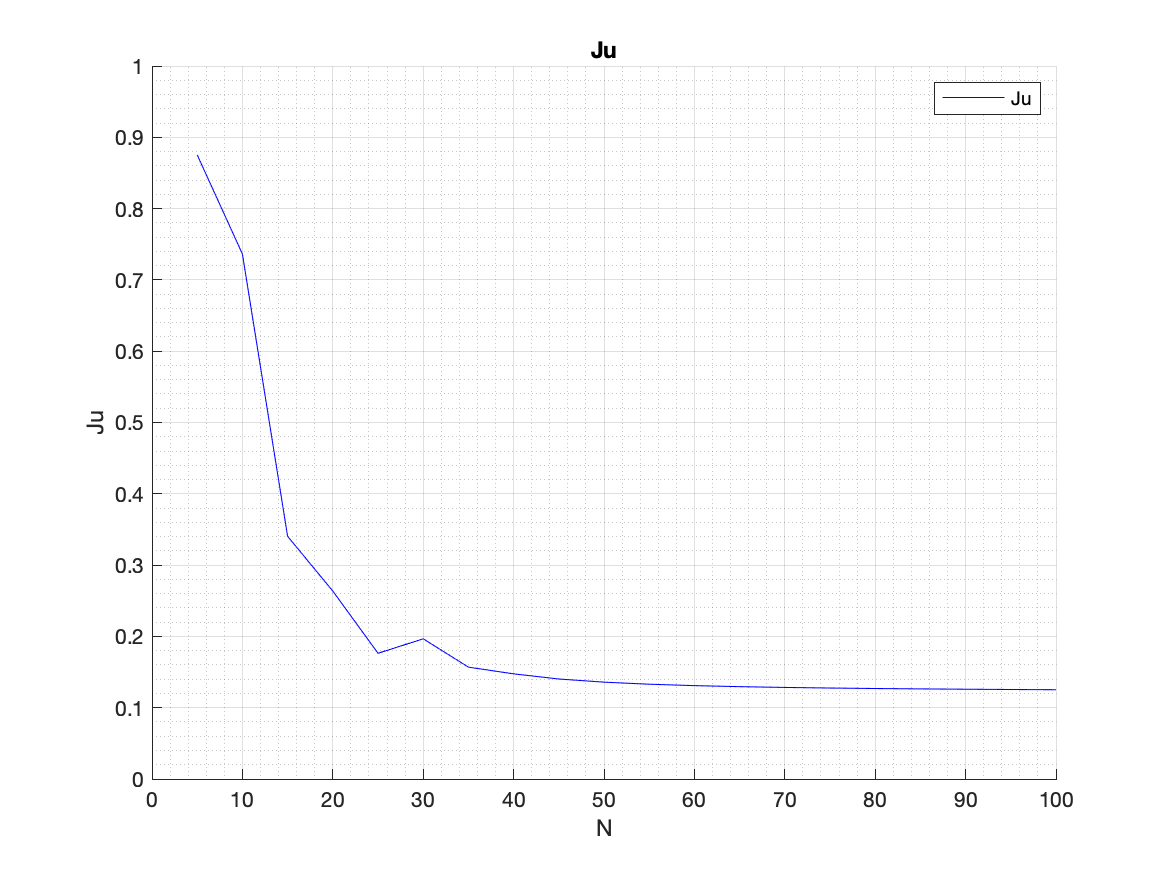
\includegraphics[width=\linewidth]{./ModelsP4_J/JuN.png} 
 \caption[Wyznaczone parametry Ju dla różnych wartości N]
{Wyznaczone parametry Ju dla różnych wartości N}
 \end{figure}

 \begin{figure} [H]
\centering
 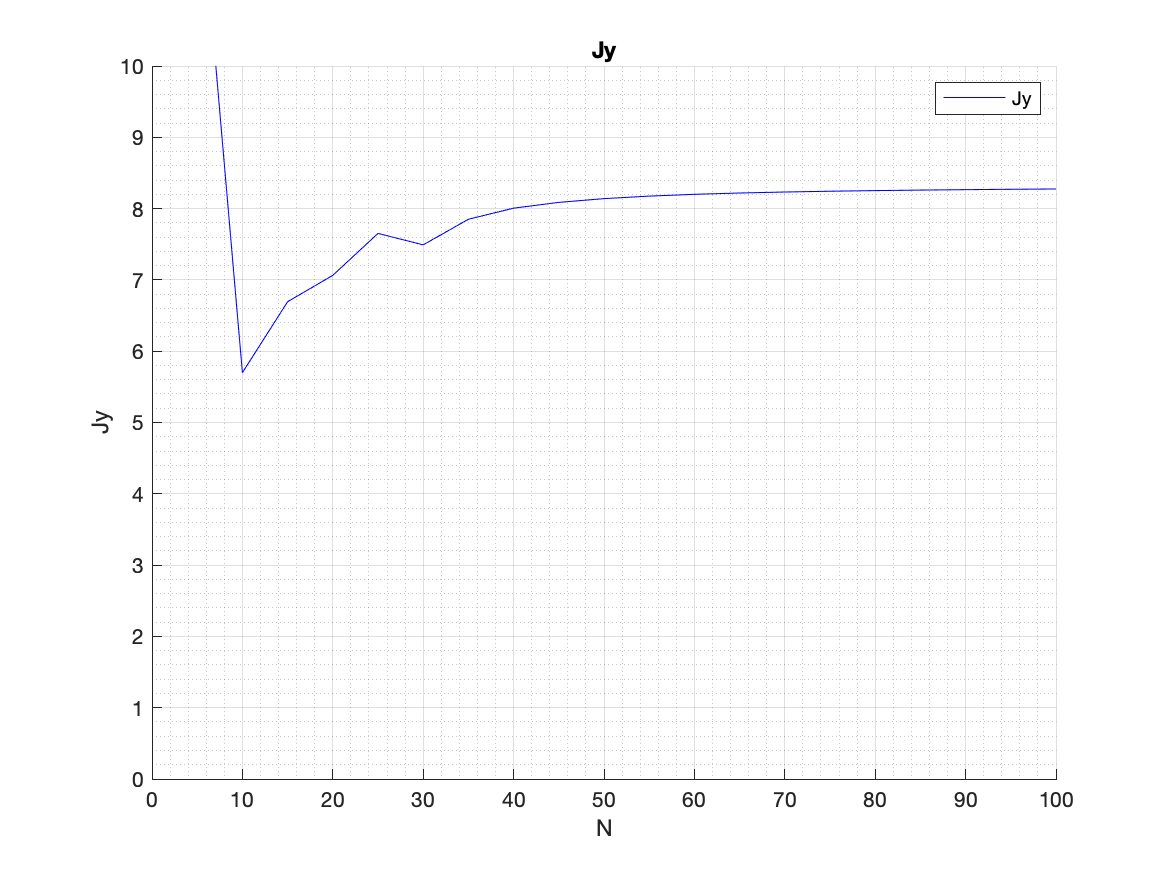
\includegraphics[width=\linewidth]{./ModelsP4_J/JyN.png} 
 \caption[Wyznaczone parametry Jy dla różnych wartości N]
{Wyznaczone parametry Jy dla różnych wartości N}
 \end{figure}
 
\begin{figure} [H]
\centering
 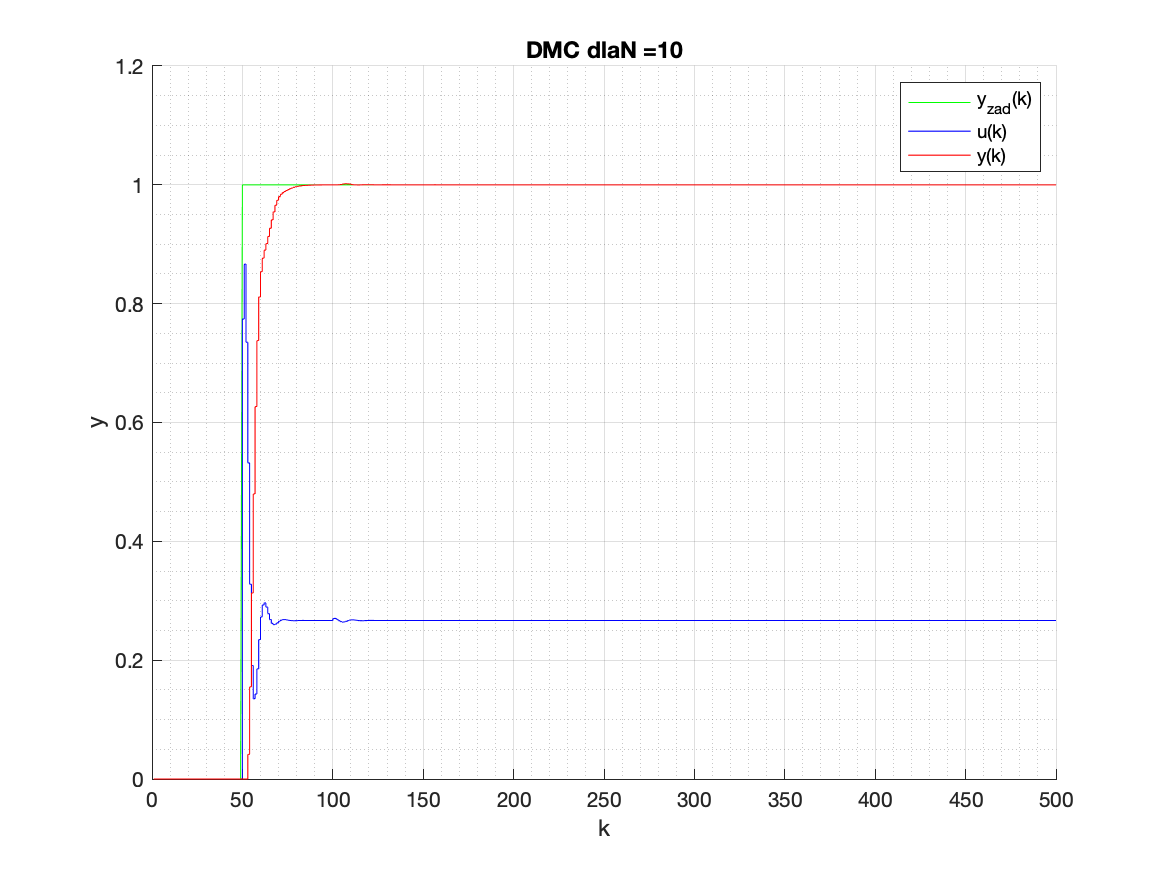
\includegraphics[width=\linewidth]{./ModelsP4_N/P4_DMC_N_10_png.png} 
 \caption[Różne wartości N - przebiegi DMC]
{Różne wartości N - przebiegi DMC}
 \end{figure}
 
 \begin{figure} [h]
\centering
 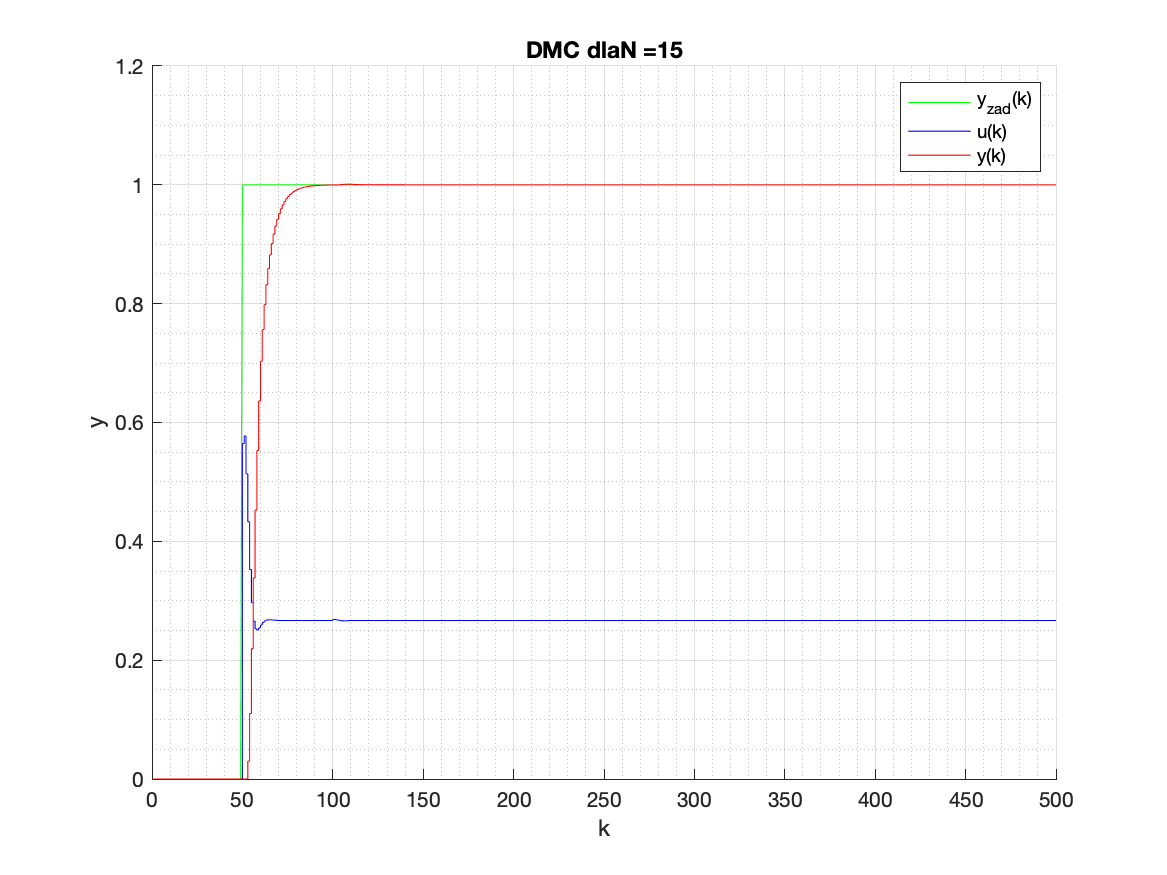
\includegraphics[width=\linewidth]{./ModelsP4_N/P4_DMC_N_15_png.png} 
 \caption[Różne wartości N - przebiegi DMC]
{Różne wartości N - przebiegi DMC}
 \end{figure}
 
 \begin{figure} [H]
\centering
  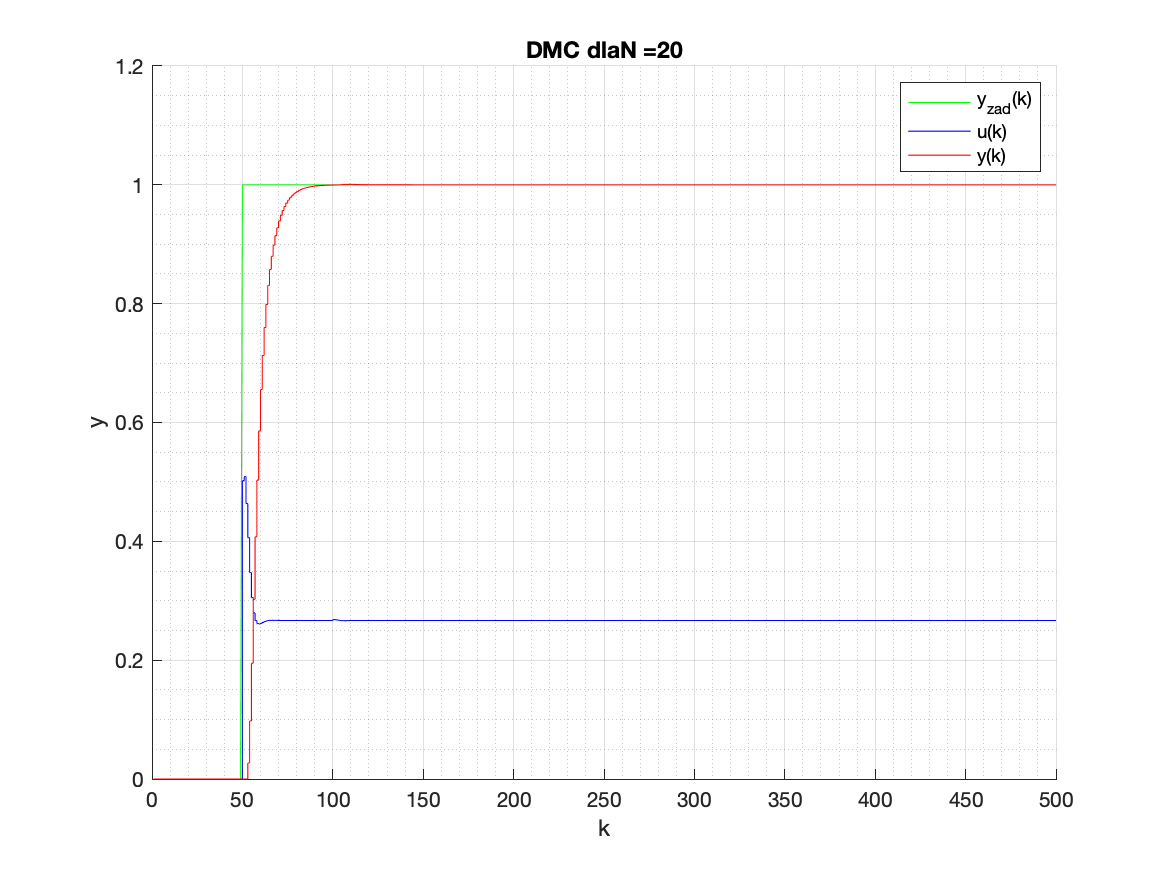
\includegraphics[width=\linewidth]{./ModelsP4_N/P4_DMC_N_20_png.png} 
 \caption[Różne wartości N - przebiegi DMC]
{Różne wartości N - przebiegi DMC}
 \end{figure}
 \begin{figure} [h]
\centering
  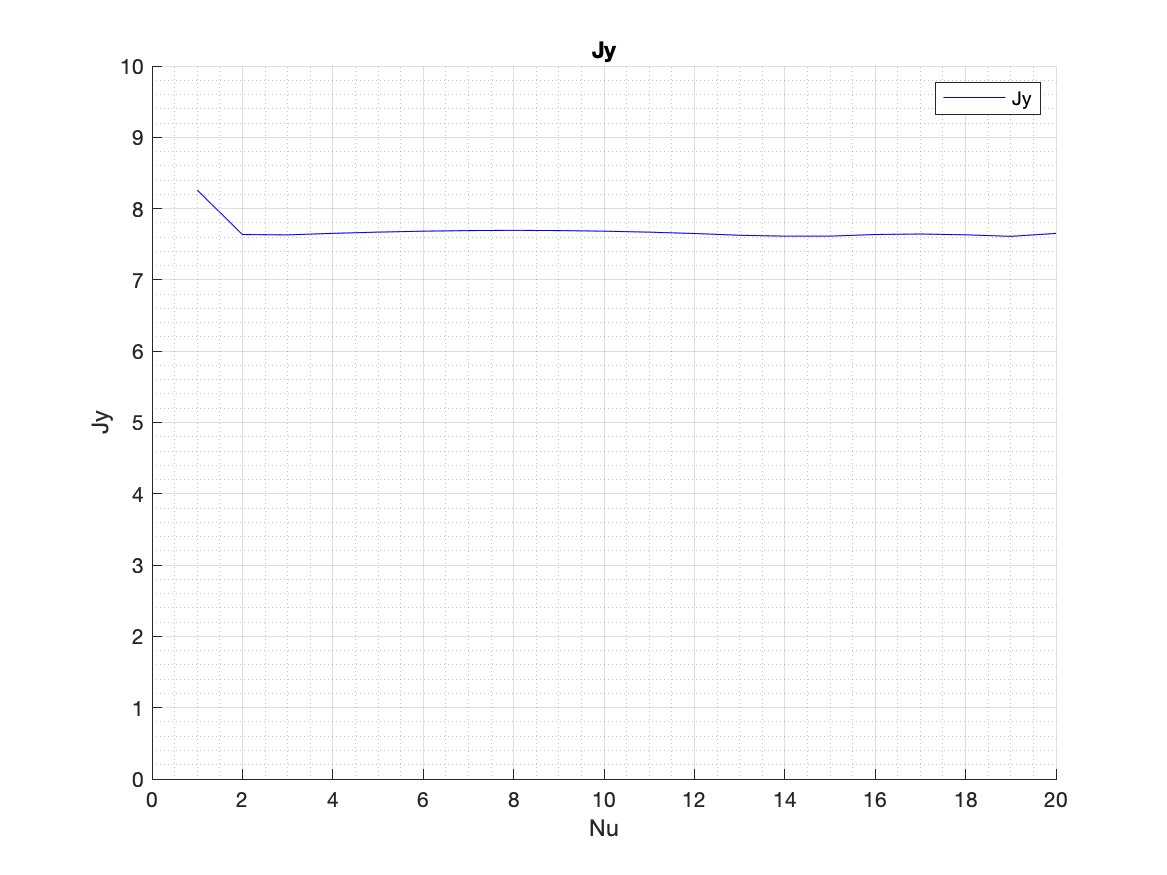
\includegraphics[width=\linewidth]{./ModelsP4_J/JyNu.png} 
 \caption[Wyznaczone parametry Jy dla różnych wartości Nu]
{Wyznaczone parametry Jy dla różnych wartości Nu}
 \end{figure}
 
 \begin{figure} [H]
\centering
 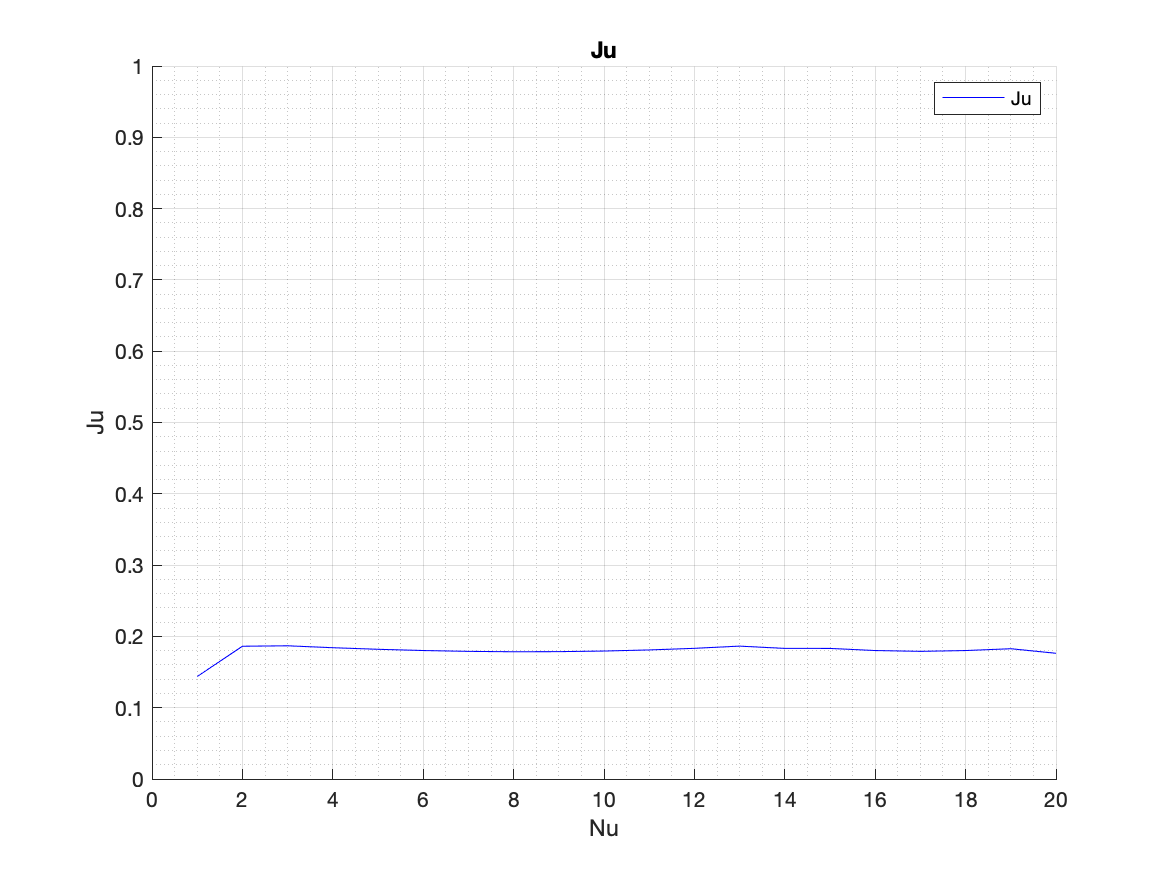
\includegraphics[width=\linewidth]{./ModelsP4_J/JuNu.png} 
 \caption[Wyznaczone parametry Ju dla różnych wartości Nu]
{Wyznaczone parametry Ju dla różnych wartości Nu}
 \end{figure}

\begin{figure} [H]
\centering
 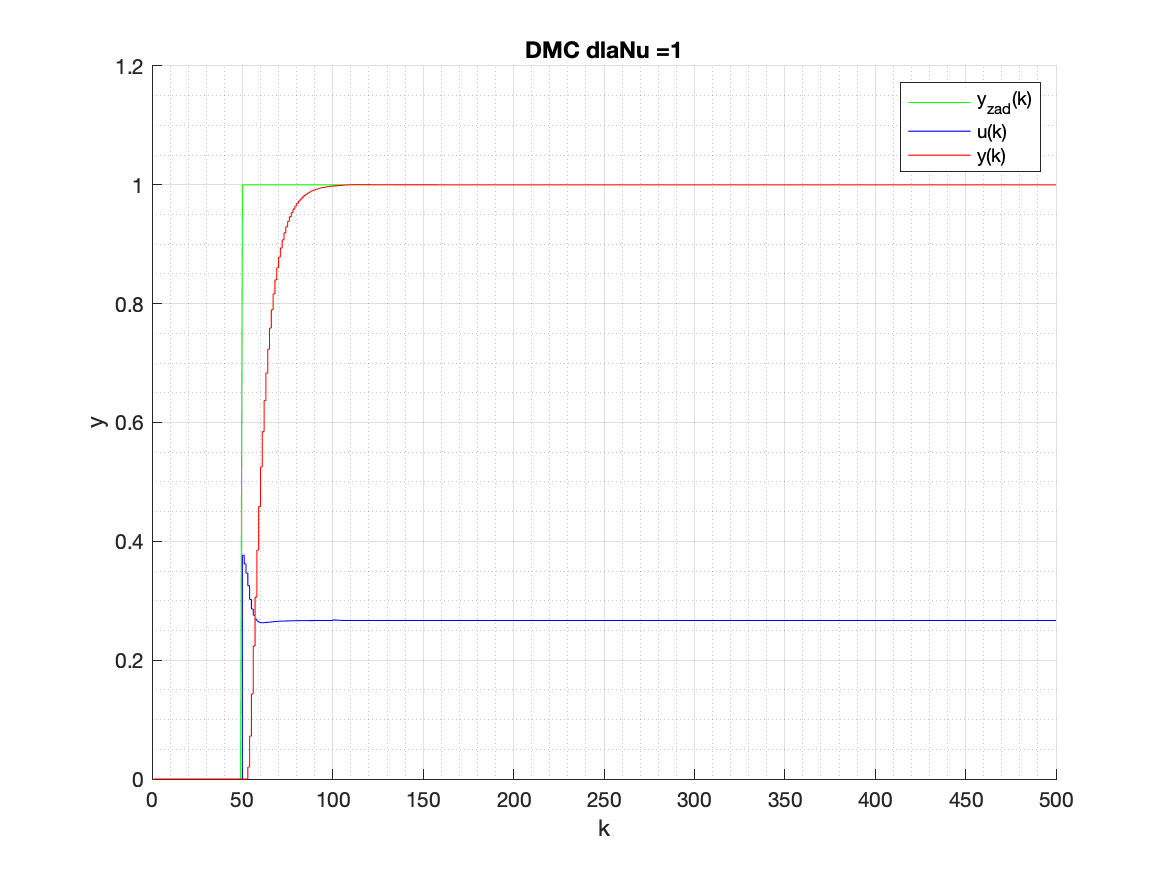
\includegraphics[width=\linewidth]{./ModelsP4_Nu/P4_DMC_Nu_1_png.png} 
 \caption[Różne wartości Nu - przebiegi DMC]
{Różne wartości Nu - przebiegi DMC}
 \end{figure}
 
 \begin{figure} [h]
\centering
 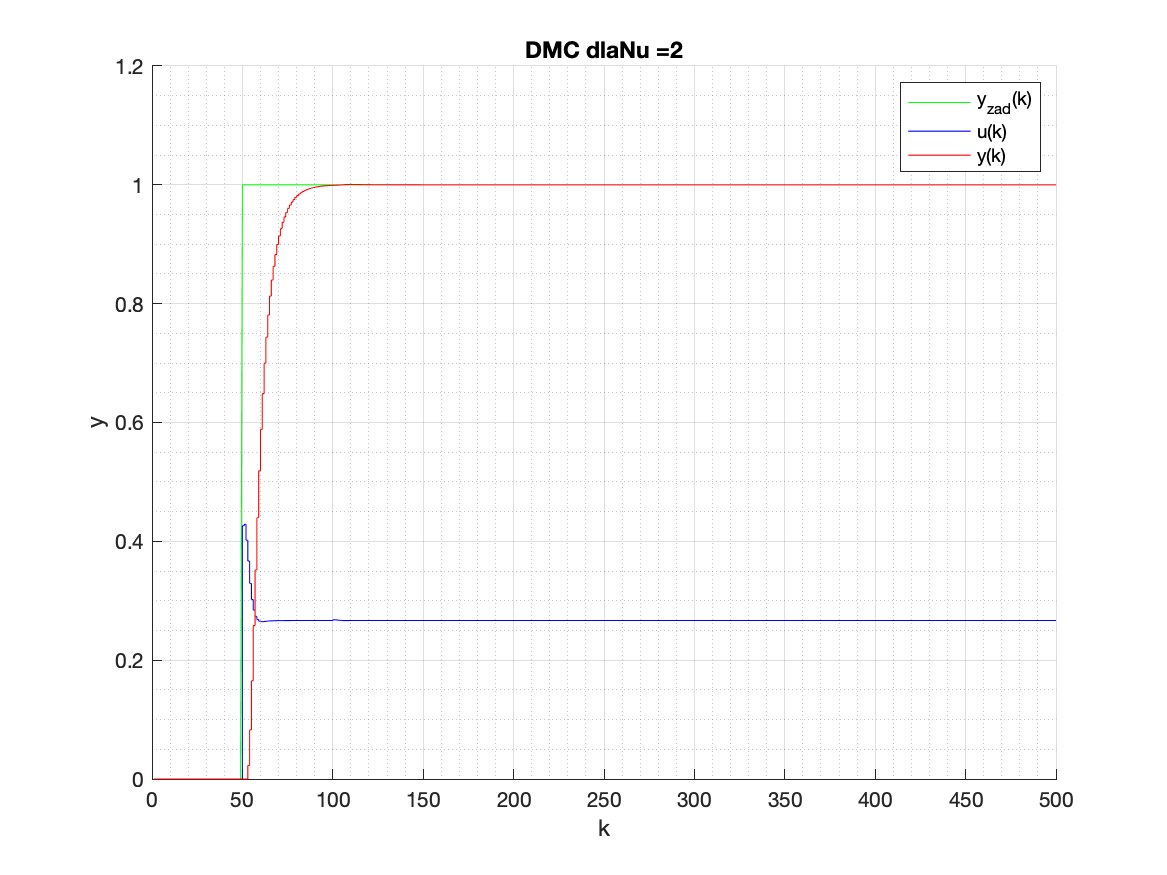
\includegraphics[width=\linewidth]{./ModelsP4_Nu/P4_DMC_Nu_2_png.png} 
 \caption[Różne wartości Nu - przebiegi DMC]
{Różne wartości Nu - przebiegi DMC}
 \end{figure}
 
 \begin{figure} [H]
\centering
  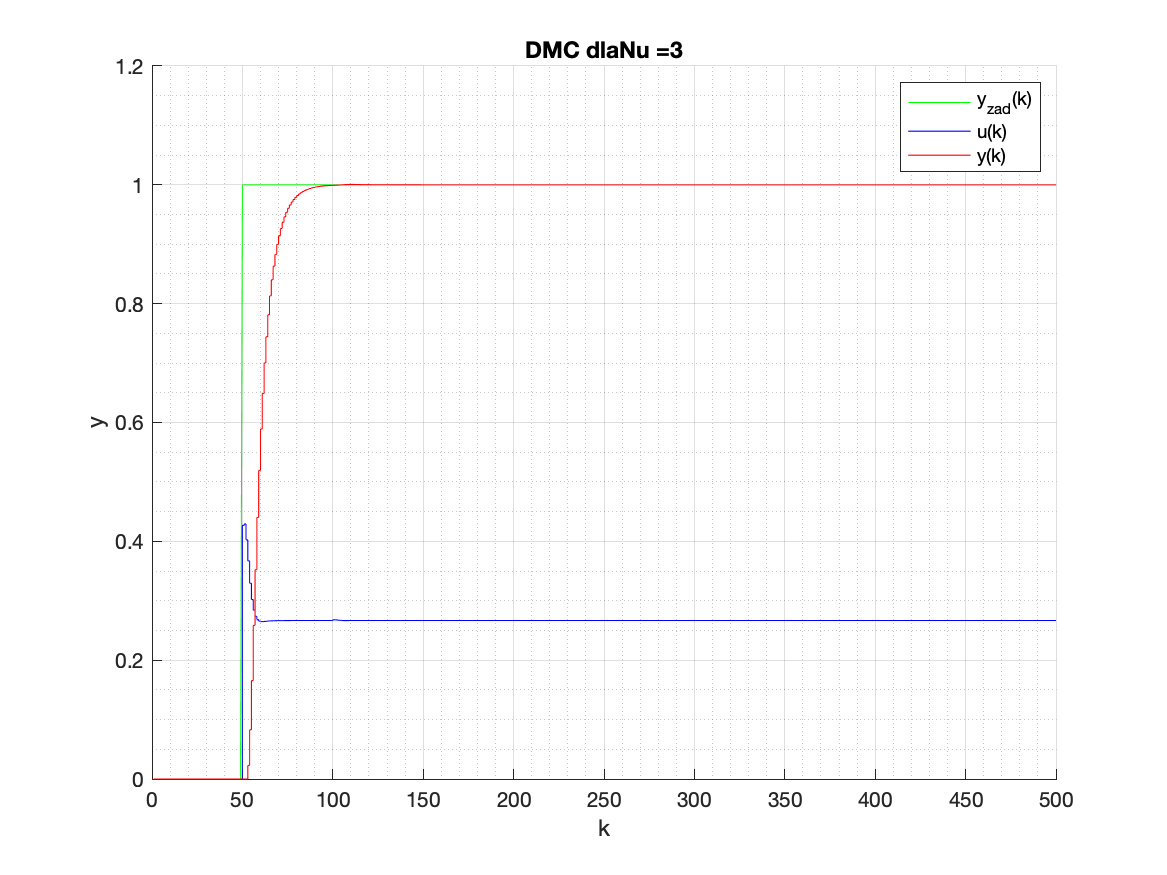
\includegraphics[width=\linewidth]{./ModelsP4_Nu/P4_DMC_Nu_3_png.png} 
 \caption[Różne wartości Nu - przebiegi DMC]
{Różne wartości Nu - przebiegi DMC}
 \end{figure}
 \begin{figure} [h]
\centering
 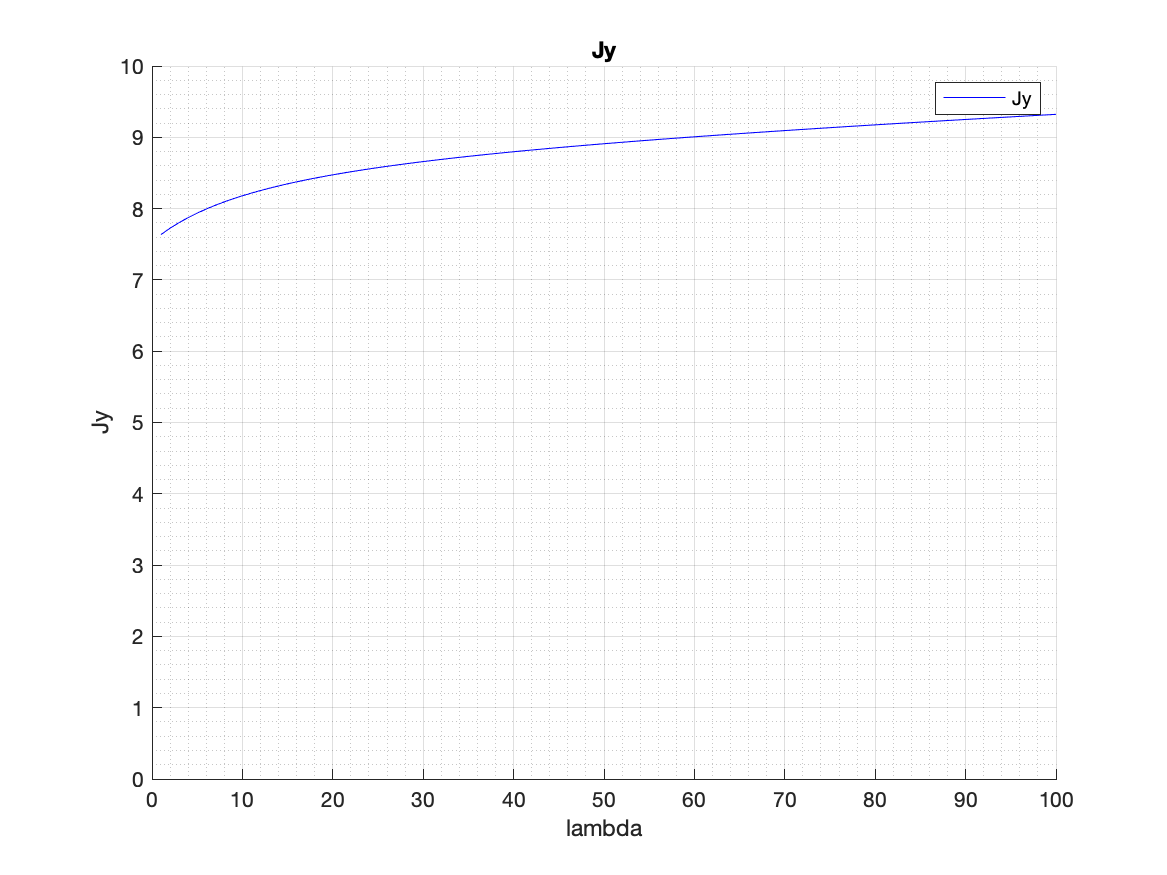
\includegraphics[width=\linewidth]{./ModelsP4_J/Jylambda.png} 
 \caption[Wyznaczone parametry Jy dla różnych wartości \lambda]
{Wyznaczone parametry Jy dla różnych wartości\( \lambda\)}
 \end{figure}
 
 \begin{figure} [H]
\centering
 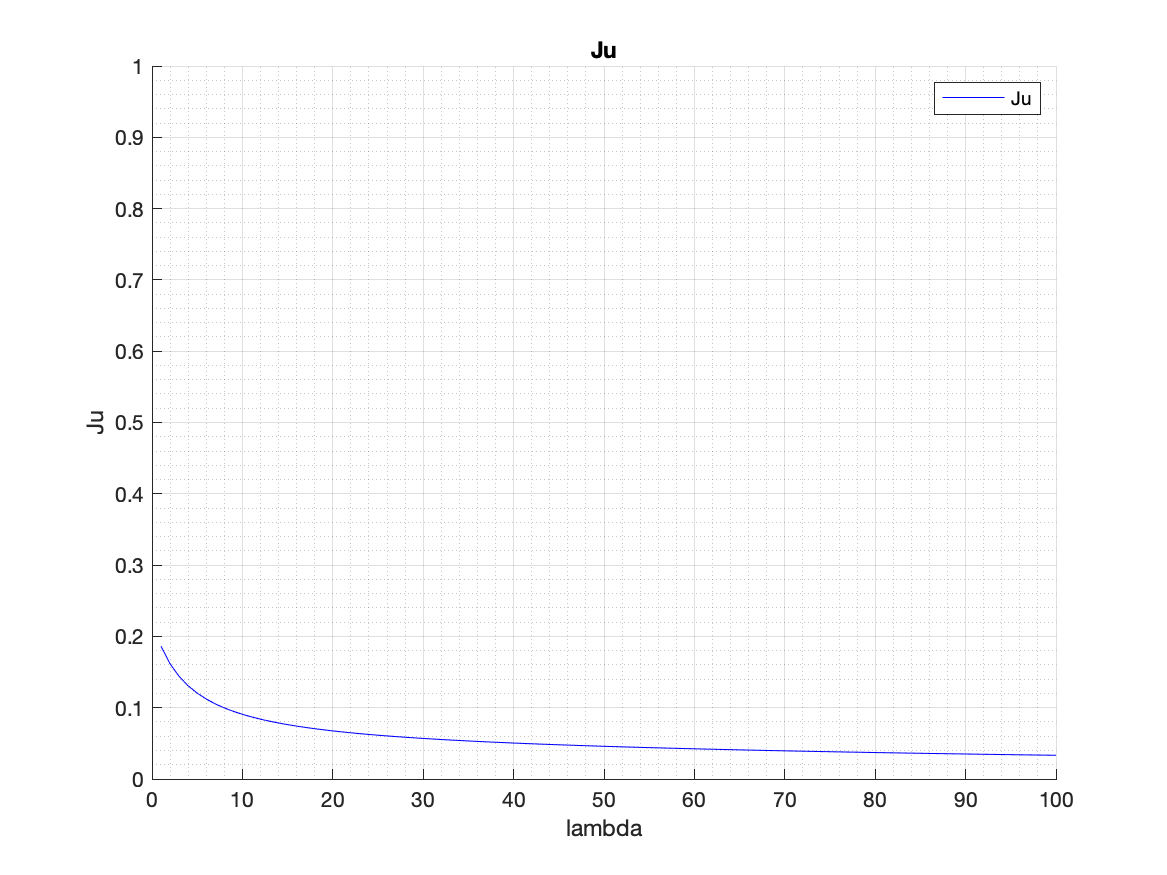
\includegraphics[width=\linewidth]{./ModelsP4_J/Julambda.png} 
 \caption[Wyznaczone parametry Ju dla różnych wartości \lambda]
{Wyznaczone parametry Ju dla różnych wartości\( \lambda\)}
 \end{figure}
 
\begin{figure} [H]
\centering
 \includegraphics[width=\linewidth]{./ModelsP4_lambda/P4_DMC_lambda_1_png.png} 
 \caption[Różne wartości lambda - przebiegi DMC]
{Różne wartości lambda - przebiegi DMC}
 \end{figure}
 
 \begin{figure} [h]
\centering
 \includegraphics[width=\linewidth]{./ModelsP4_lambda/P4_DMC_lambda_2_png.png} 
 \caption[Różne wartości lambda - przebiegi DMC]
{Różne wartości lambda - przebiegi DMC}
 \end{figure}
 
 \begin{figure} [H]
\centering
  \includegraphics[width=\linewidth]{./ModelsP4_lambda/P4_DMC_lambda_3_png.png} 
 \caption[Różne wartości lambda - przebiegi DMC]
{Różne wartości lambda - przebiegi DMC}
 \end{figure}
\newpage
Dla każdego parametru starałem się wybrać odpowiednią wartość.Dla D zdecydowałem się na wartość D = 50 jako że wtedy wszystkie błędy ostatecznie się wygładzają i dla kolejnych wartości symulacji wyniki są odpowiednie.W związku z błędem w obliczeniach wykresy J były źle obliczane i nie mogłem się nimi posiłkować, teraz dysponując tymi danymi rozważyłbym wybranie D = 40 czy nawet 35, jako że drobne zakłócenia nadal występujące mają ostatecznie dość mały wpływ na jakość sterowania. Stosując podobną logikę wybrałem wartości N = 15 jako że oferuje dobry balans pomiędzy parametrami Ju i Jy, dla Nu okazało się że już dla wartości 2 kolejna wersja modelu nie przynosi znaczącej poprawy, natomiast dla lambdy zdecydowałem że \( \lambda = 3 \) daje odpowiednio dokładne wyniki.
\\* \\*Kod Do wyznaczenia p. 4: \\

\lstinputlisting{P4_Determining_D.m} 
\lstinputlisting{P4_Determining_Lambda.m} 
\lstinputlisting{P4_Determining_N.m} 
\lstinputlisting{P4_Determining_Nu.m} 

Ogólny algorytm DMC bez ograniczeń : \\
 \lstinputlisting{DMCnoLimit.m} 
\newpage
\item DMC z zakłóceniem\\
W wersji DMC z wprowadzonym zakłóceniem badałem zakres skoku zakłóceń od 0 do 5, i wyniki były bardzo powtarzalne.Kształt sygnału był taki sam dla wszystkich wartości, a amplituda sygnału wyjściowego wydaje się być proporcjonalna do skali zakłócenia
\lstinputlisting{P5.m} 
Przykładowe wykresy :\\
 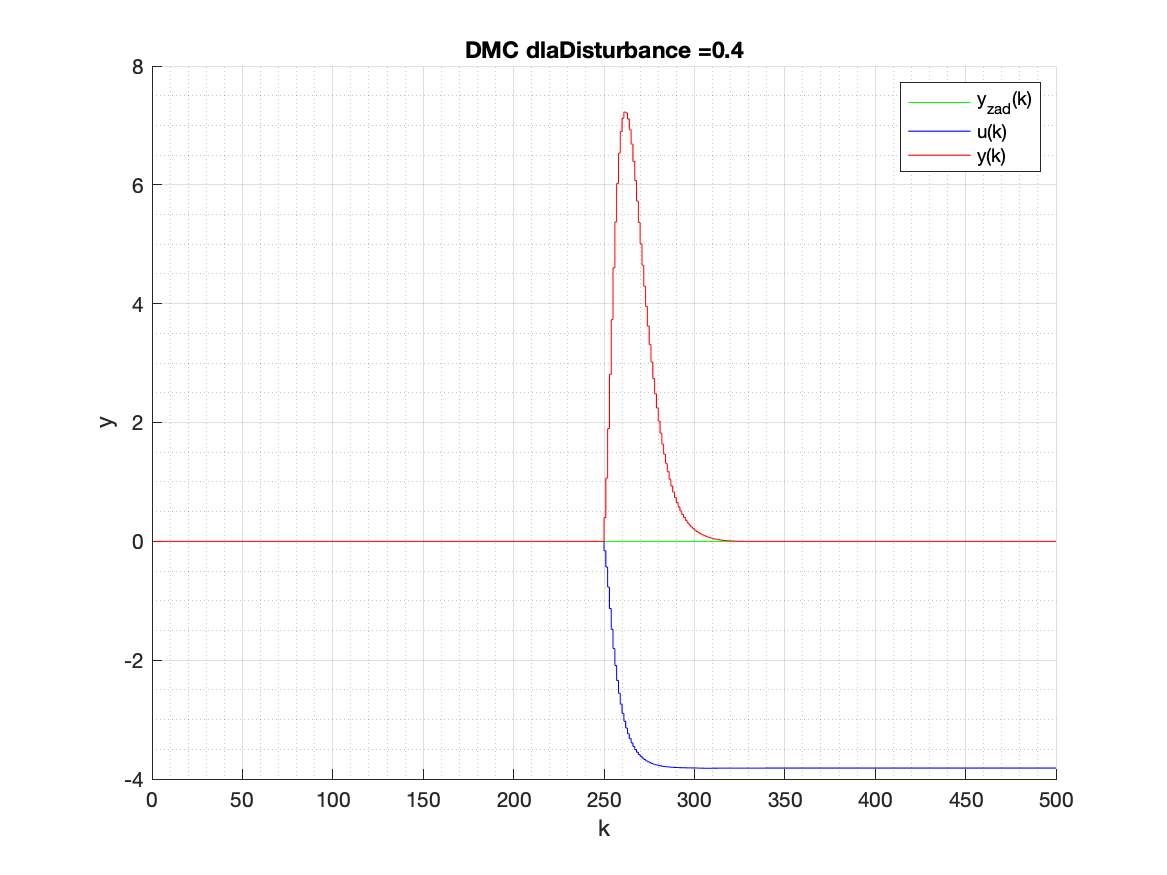
\includegraphics[width=\linewidth]{./ModelsP4_Disturbance/P4_DMC_Disturbance_0_4_png.png} 
  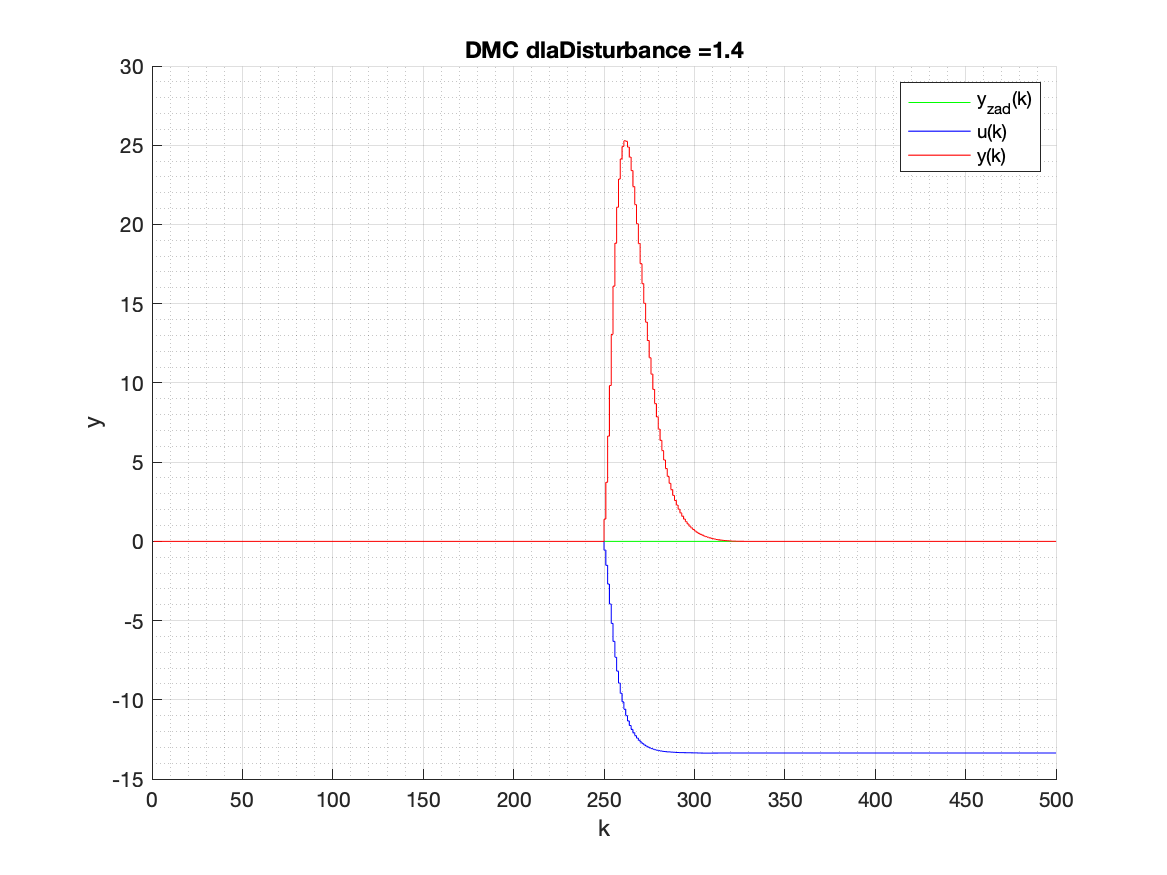
\includegraphics[width=\linewidth]{./ModelsP4_Disturbance/P4_DMC_Disturbance_1_4_png.png} 
   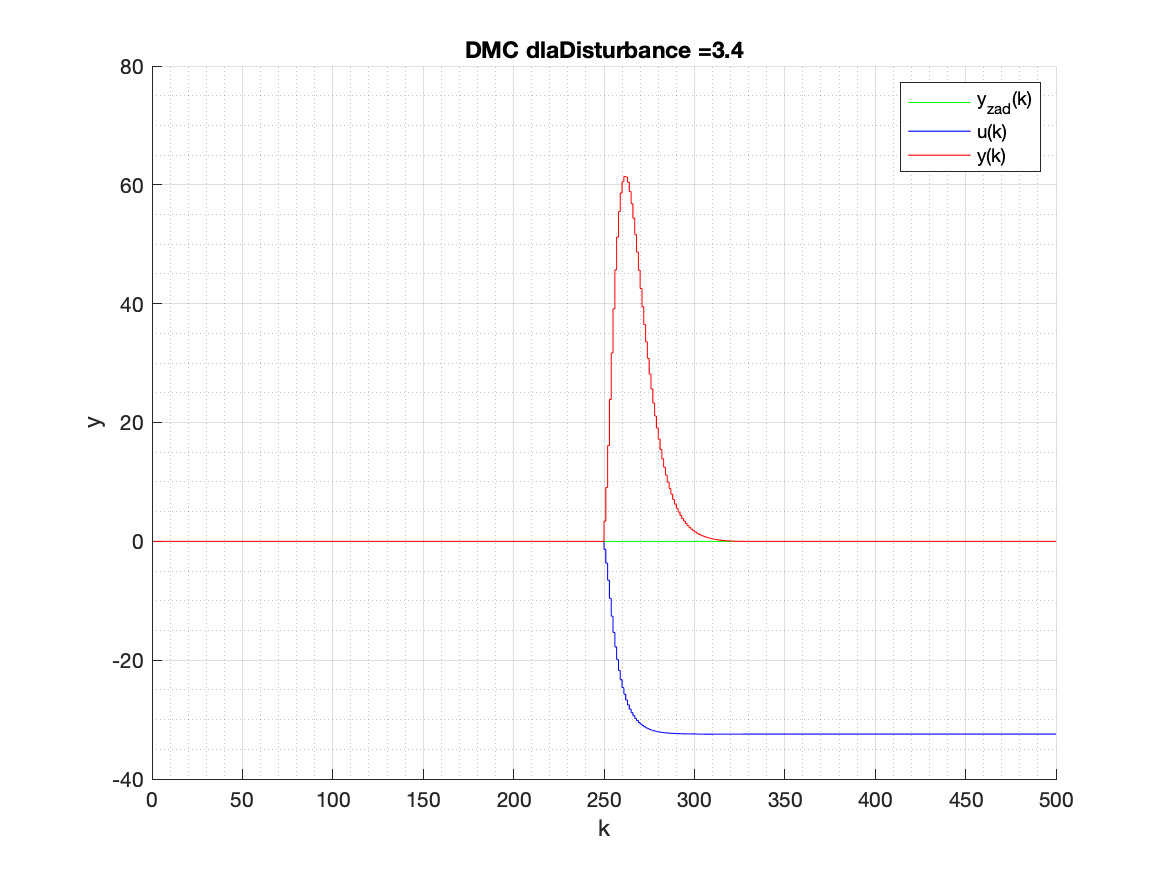
\includegraphics[width=\linewidth]{./ModelsP4_Disturbance/P4_DMC_Disturbance_3_4_png.png} 
    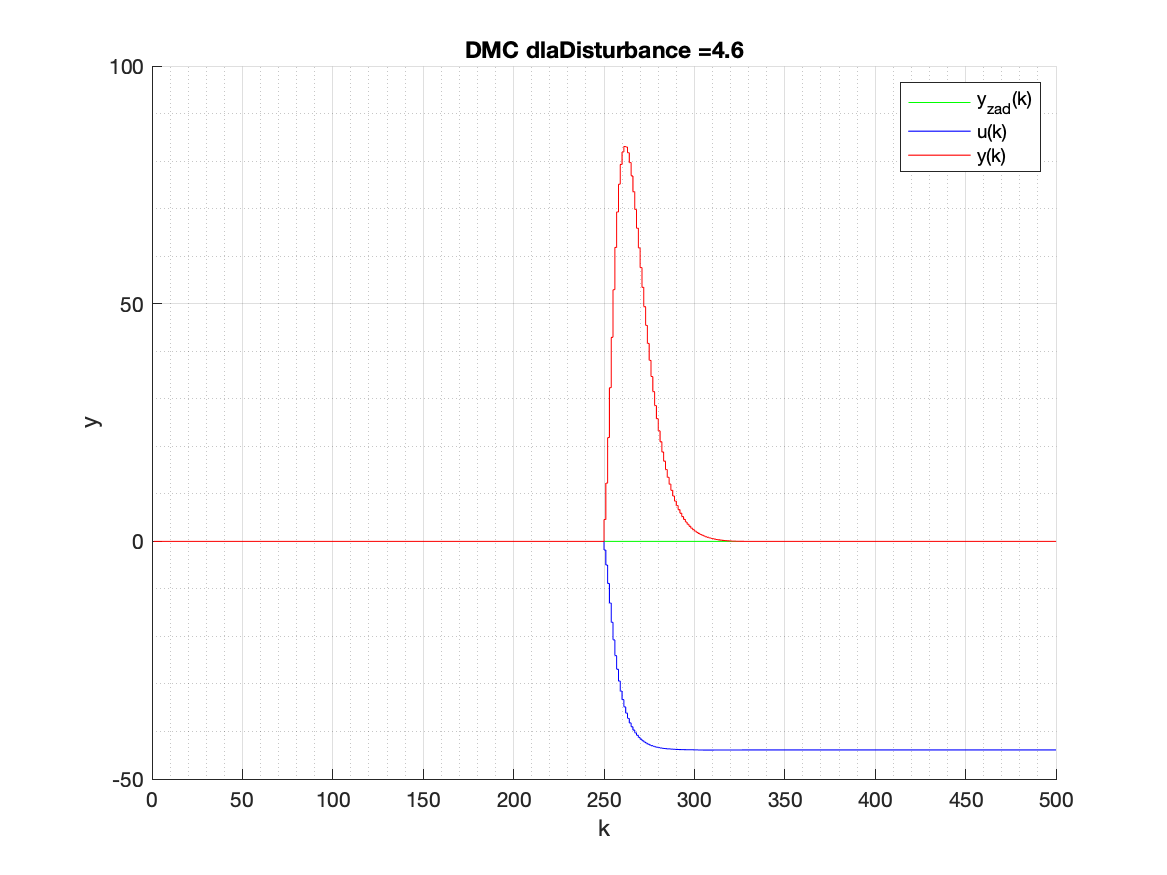
\includegraphics[width=\linewidth]{./ModelsP4_Disturbance/P4_DMC_Disturbance_4_6_png.png} 
   \newpage

\item Ograniczenia w symulacji DMC
\begin{itemize}

 \item Ograniczenie wartości U \\
 Dla ograniczeń sygnału sterującego wybrałem wartość optymalną umax = 0.27.Dalsze zwiększanie tej wartości nie ma dużego wpływu na regulacje, za to zmniejszanie szybko prowadzi do uniemożliwienia sensownej regulacji.
 Kod : \\
 \lstinputlisting{P6_1.m} 
   Wykresy przykładowe:\\
 
 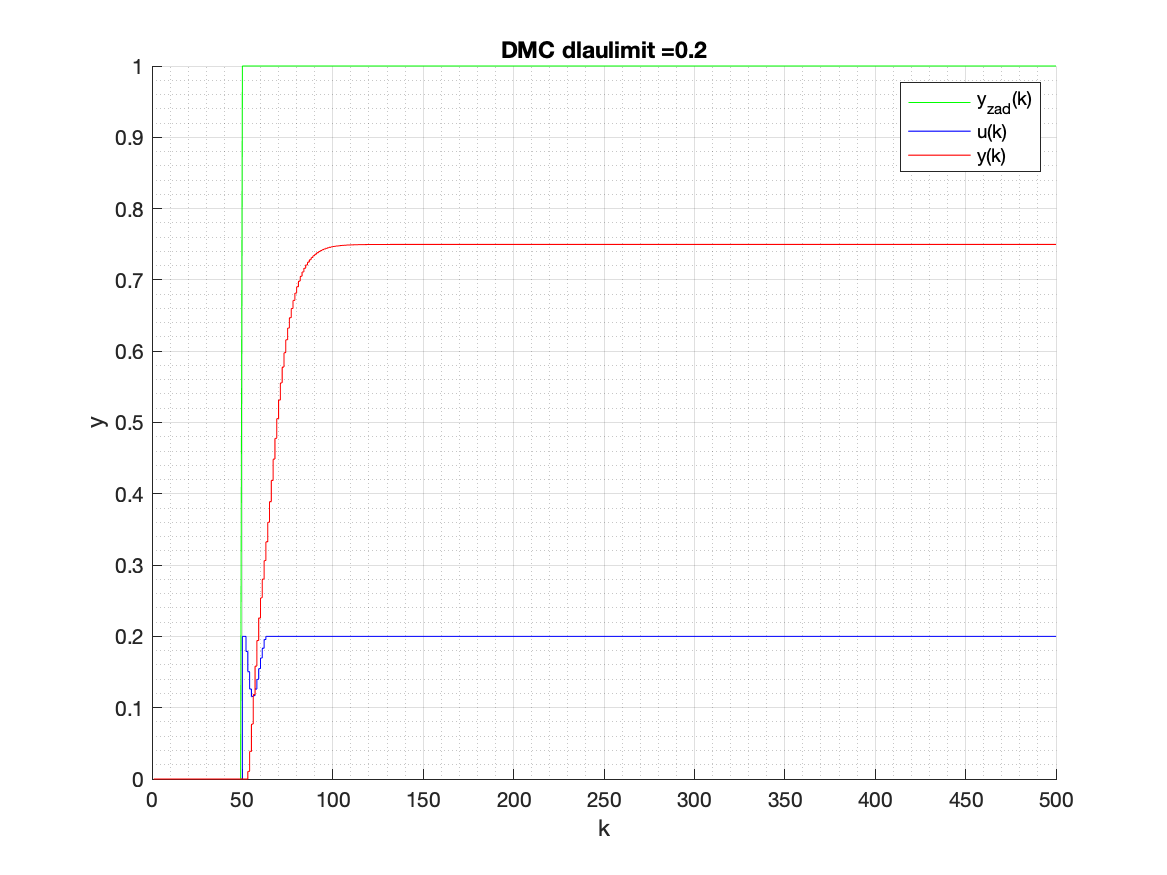
\includegraphics[width=\linewidth]{./ModelsP6_ulimit/P4_DMC_ulimit_0_2_png.png} 
 
 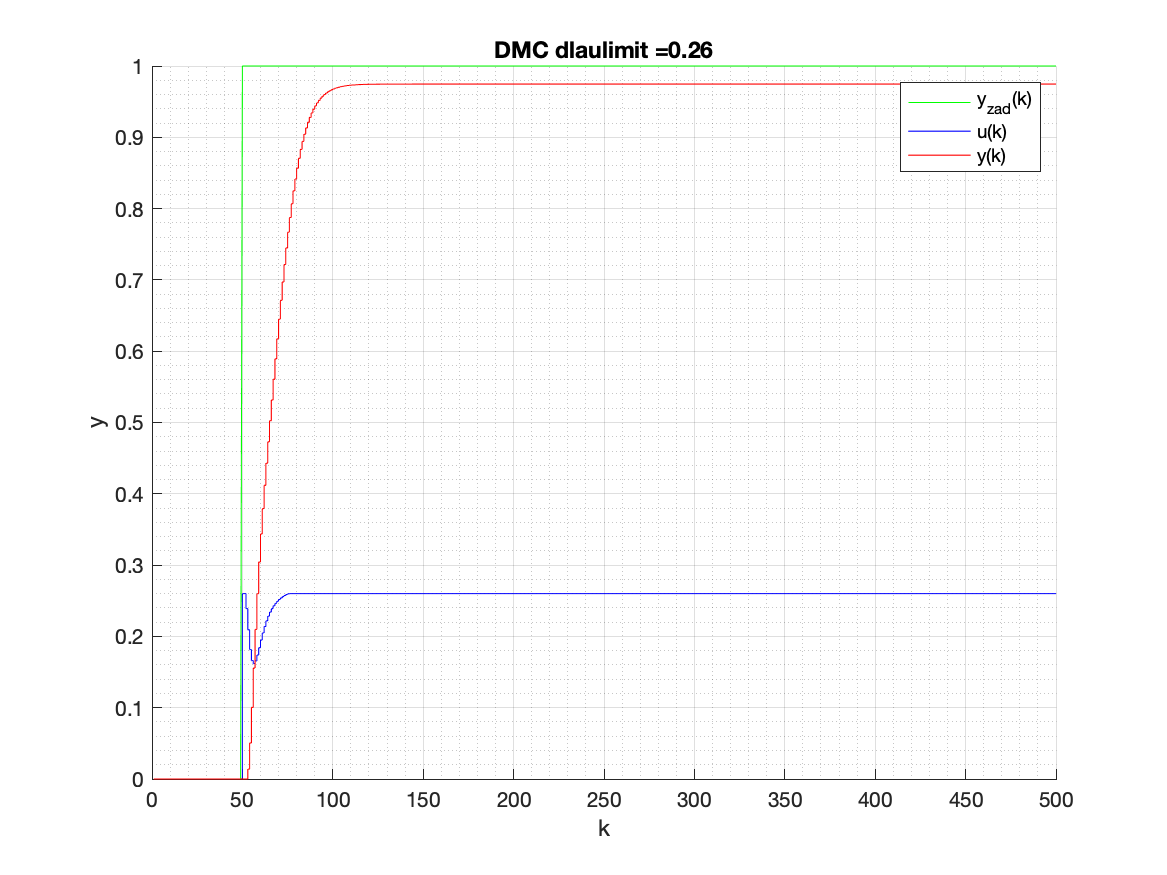
\includegraphics[width=\linewidth]{./ModelsP6_ulimit/P4_DMC_ulimit_0_26_png.png} 
 
 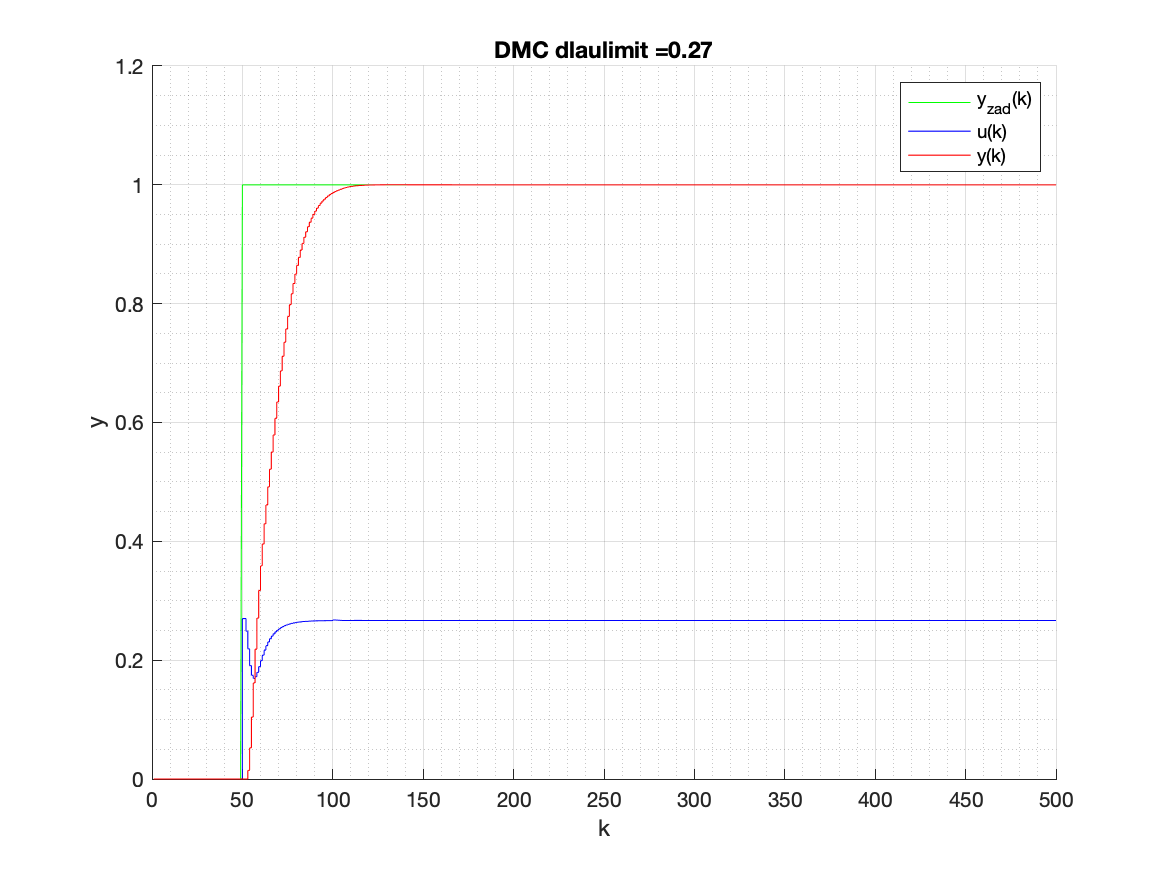
\includegraphics[width=\linewidth]{./ModelsP6_ulimit/P4_DMC_ulimit_0_27_png.png} 
 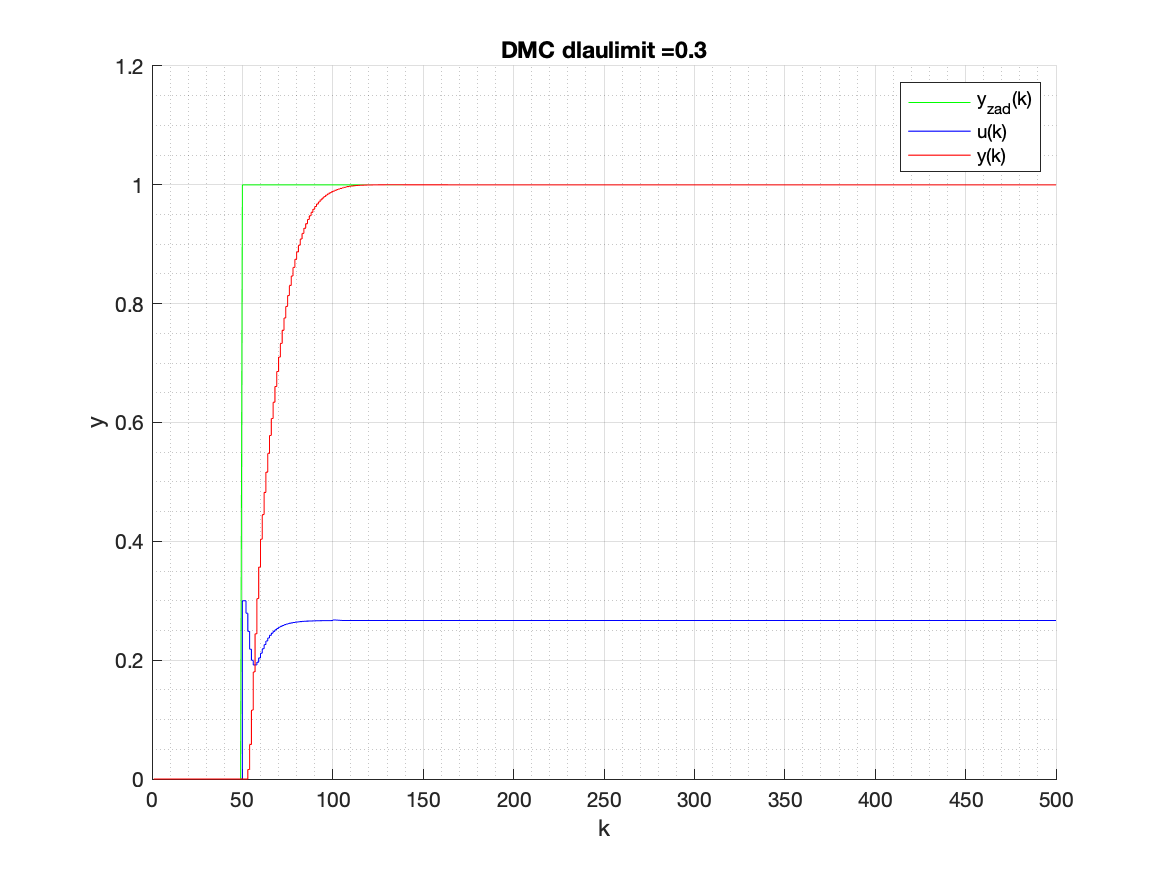
\includegraphics[width=\linewidth]{./ModelsP6_ulimit/P4_DMC_ulimit_0_3_png.png} 
 \item Ograniczenie wartości dU \\
 Dla ograniczeń przyrostów wymierny wpływ zaczyna się wygładzać dla współczynnika około 0.05, a jako odpowiednie ograniczenie wybrałem 0.09
 Kod : \\
   \lstinputlisting{P6_2.m} 
   \newpage
   Wykresy przykładowe:\\

 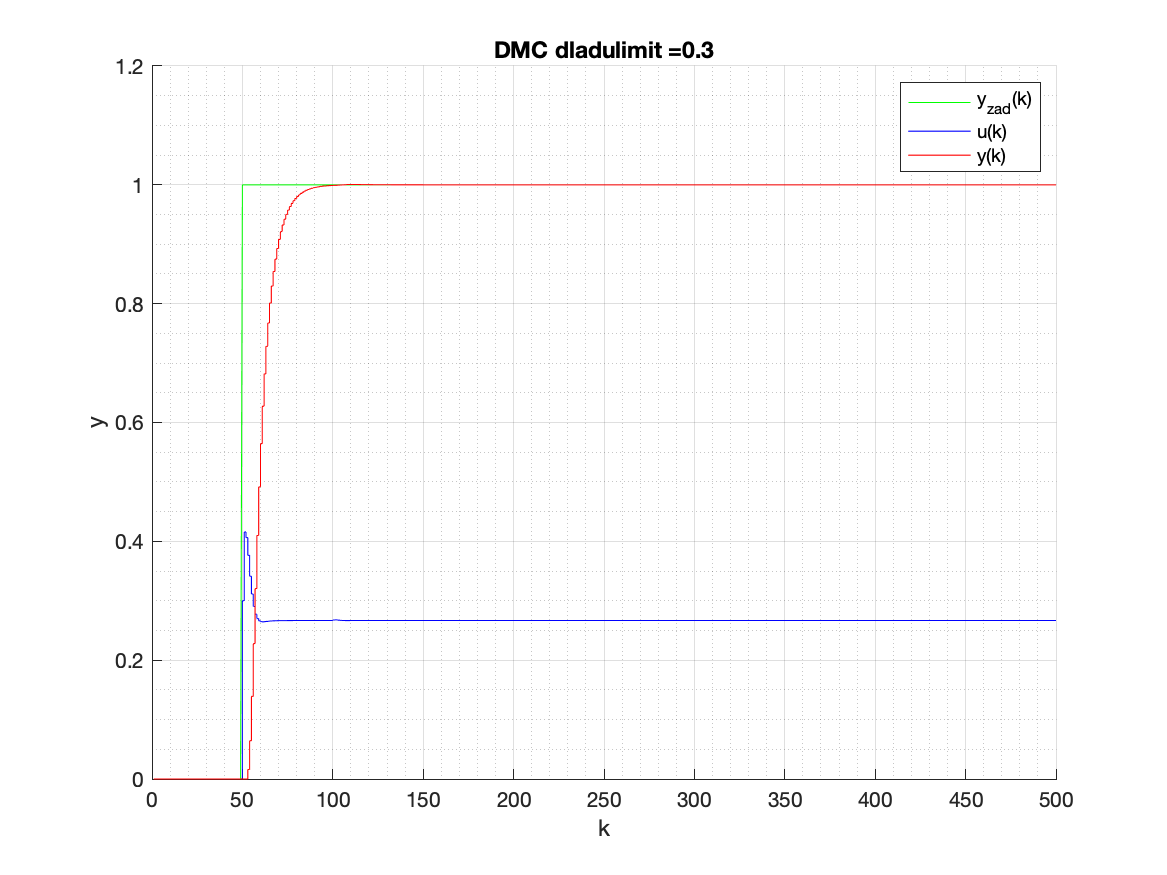
\includegraphics[width=\linewidth]{./ModelsP6_dulimit/P4_DMC_dulimit_0_3_png.png} 

 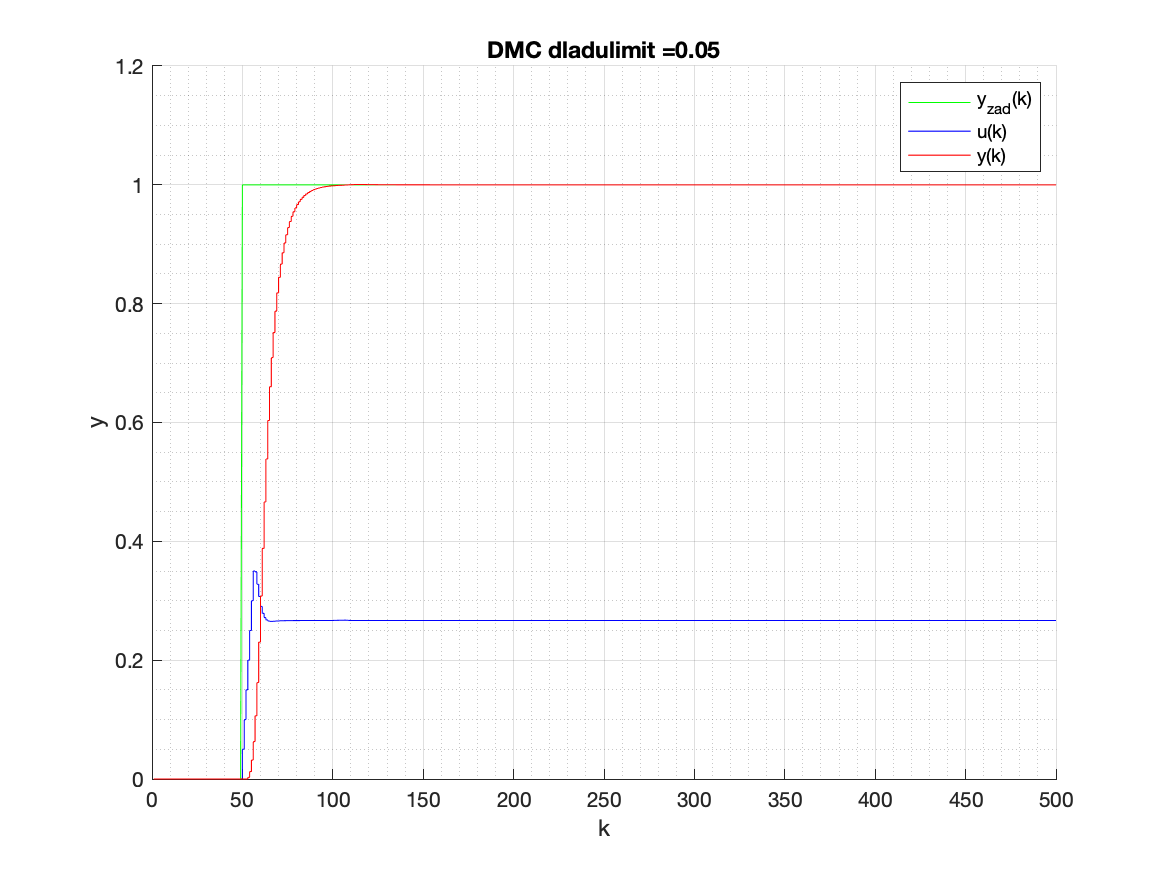
\includegraphics[width=\linewidth]{./ModelsP6_dulimit/P4_DMC_dulimit_0_05_png.png} 
 
 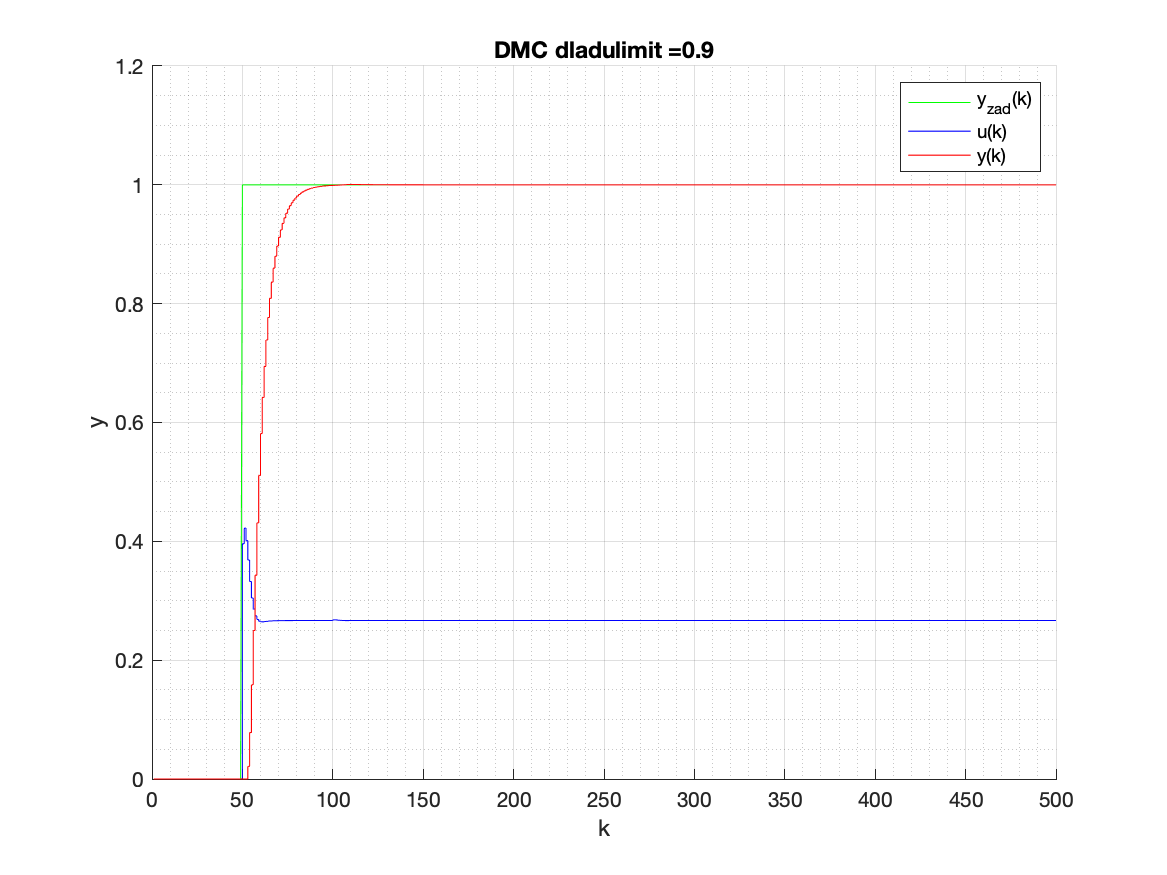
\includegraphics[width=\linewidth]{./ModelsP6_dulimit/P4_DMC_dulimit_0_9_png.png} 

  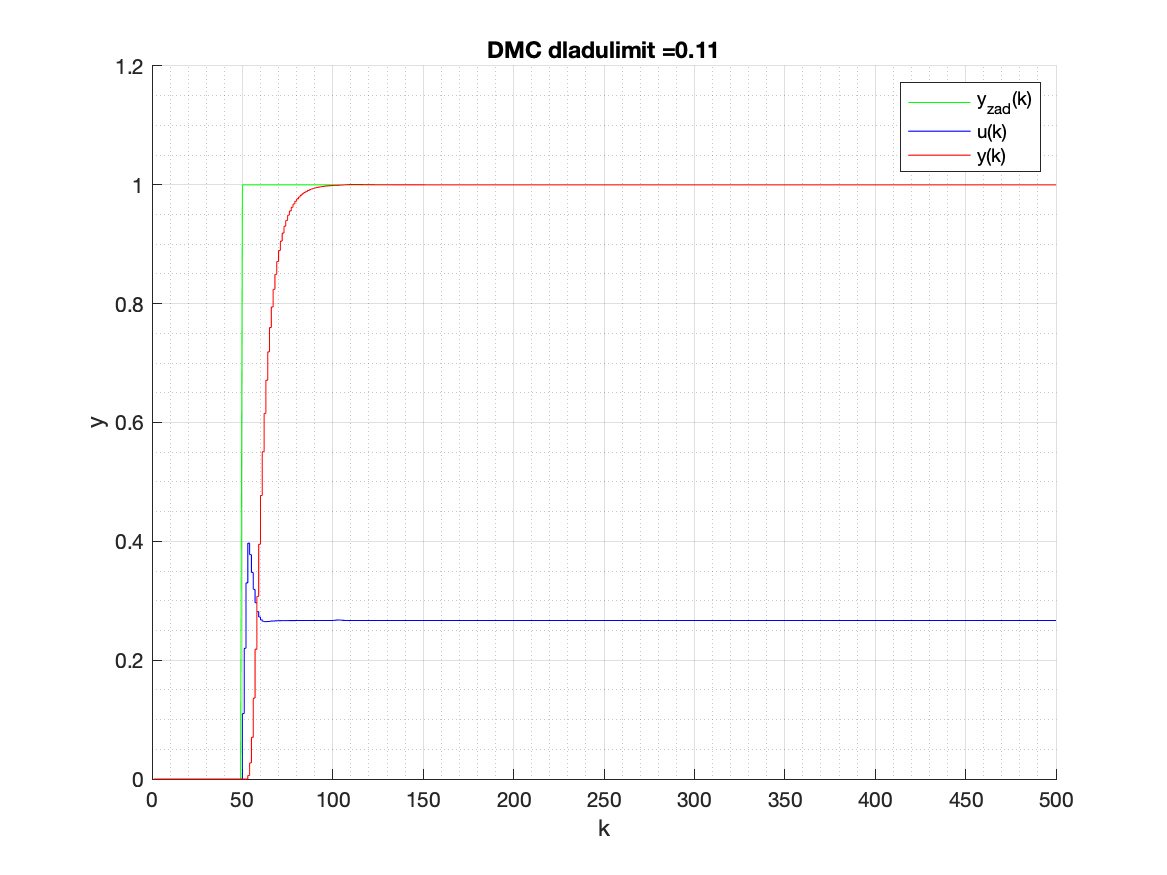
\includegraphics[width=\linewidth]{./ModelsP6_dulimit/P4_DMC_dulimit_0_11_png.png} 


  \item Ograniczenie wartości U oraz dU \\
 
  Wybrane wartosci : dulimit = 0.27 , dlimit = 0.09 \\Jak widać na wykresie sterowanie jest skuteczne dla wybranych wartości ograniczeń
Wykres:\\

     \begin{figure} [H]
\centering
 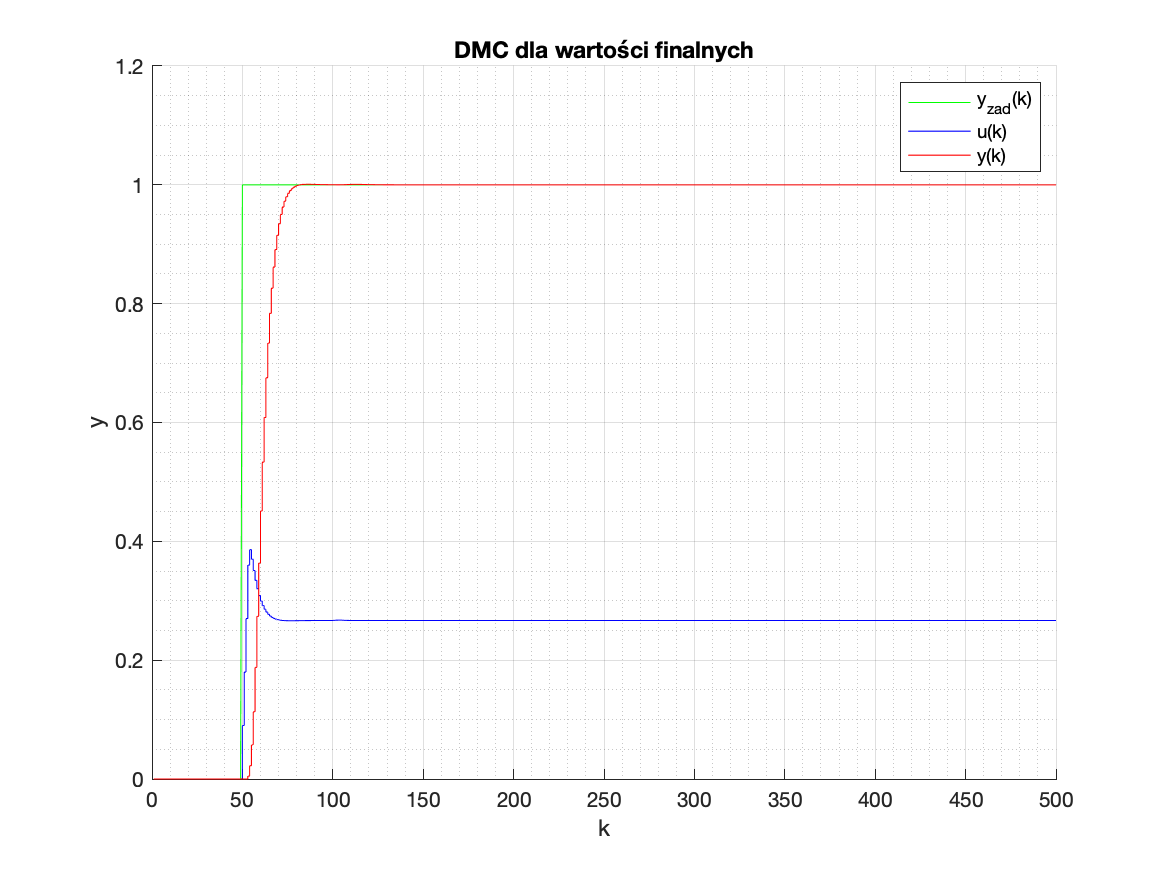
\includegraphics[width=\linewidth]{./P6_3_DMC_Koncowe_.png} 
 \caption{Sterowanie dla dulimit = 0,27 , dlimit = 0,09  }
 \end{figure}
  Kod : \\
  \lstinputlisting{P6_3.m} 


\end{itemize}
\item Zadanie dodatkowe\\
Jak widać na wykresach dla wartości \( \alpha\) na początku system DMC dobrze radzi sobie z kompensowaniem błędów. Dla  \( \alpha = 1,5 \) zaczynamy obserwować przeregulowanie które szybko staje się widoczne.Dla wartości krytycznej  \( \alpha = 4.4 \) system przestaje być zbieżny oraz spełniać swoją rolę
 
 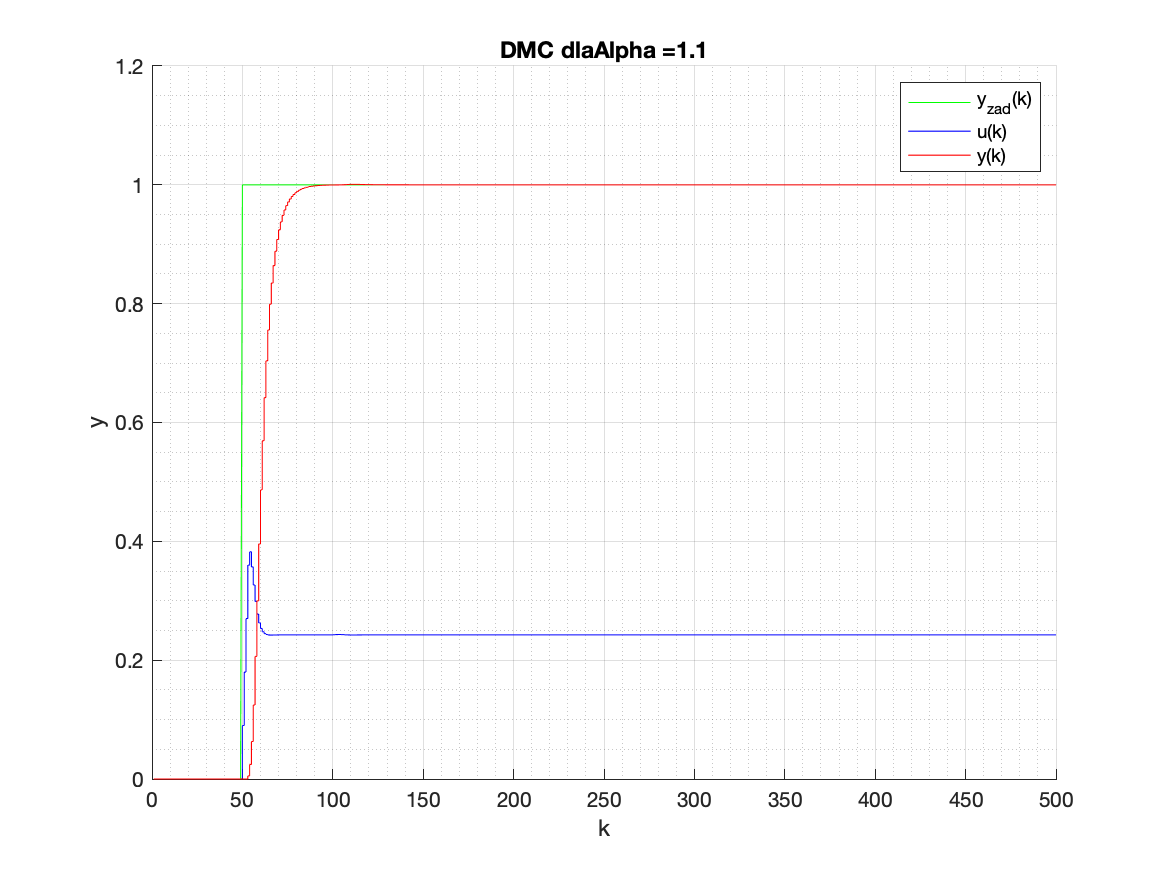
\includegraphics[width=\linewidth]{./ModelsDodatkowe_Alpha/P4_DMC_Alpha_1_1_png.png} 
 
 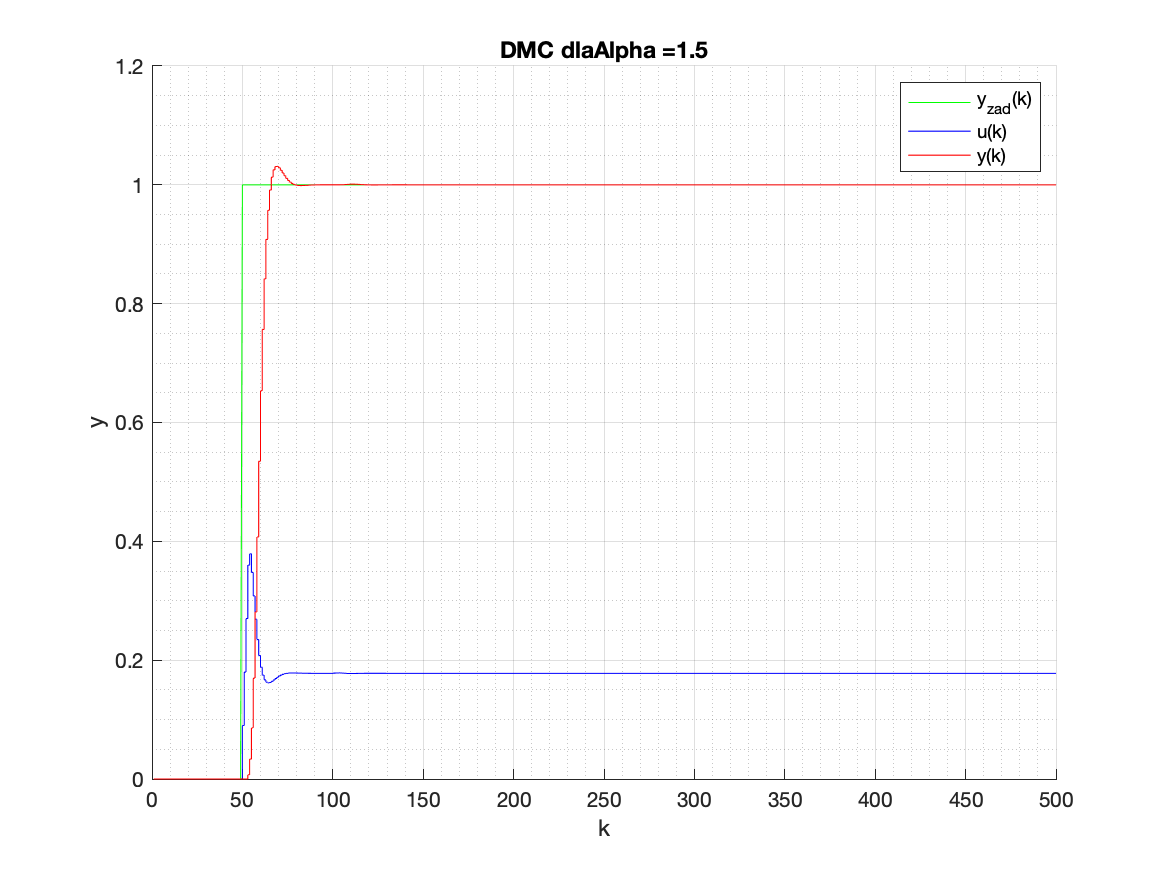
\includegraphics[width=\linewidth]{./ModelsDodatkowe_Alpha/P4_DMC_Alpha_1_5_png.png} 
 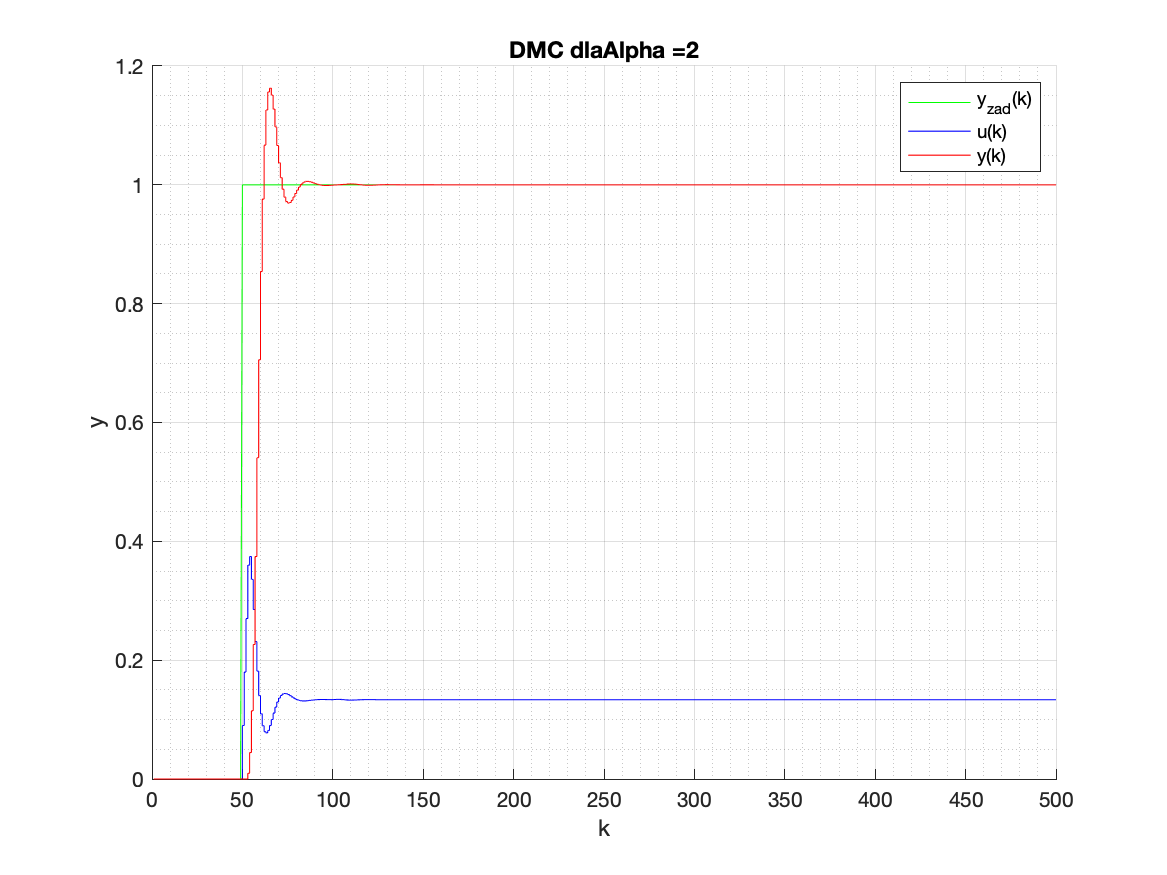
\includegraphics[width=\linewidth]{./ModelsDodatkowe_Alpha/P4_DMC_Alpha_2_png.png} 
 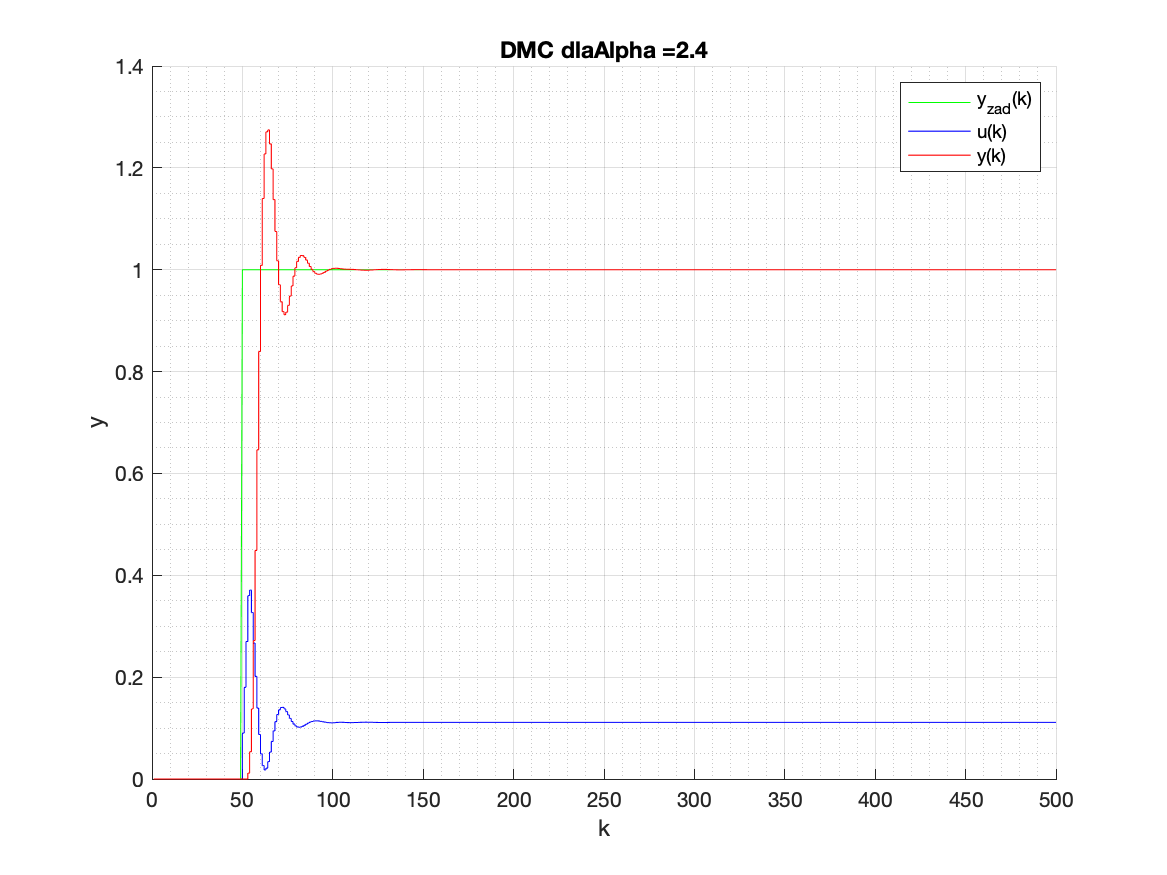
\includegraphics[width=\linewidth]{./ModelsDodatkowe_Alpha/P4_DMC_Alpha_2_4_png.png} 
 
 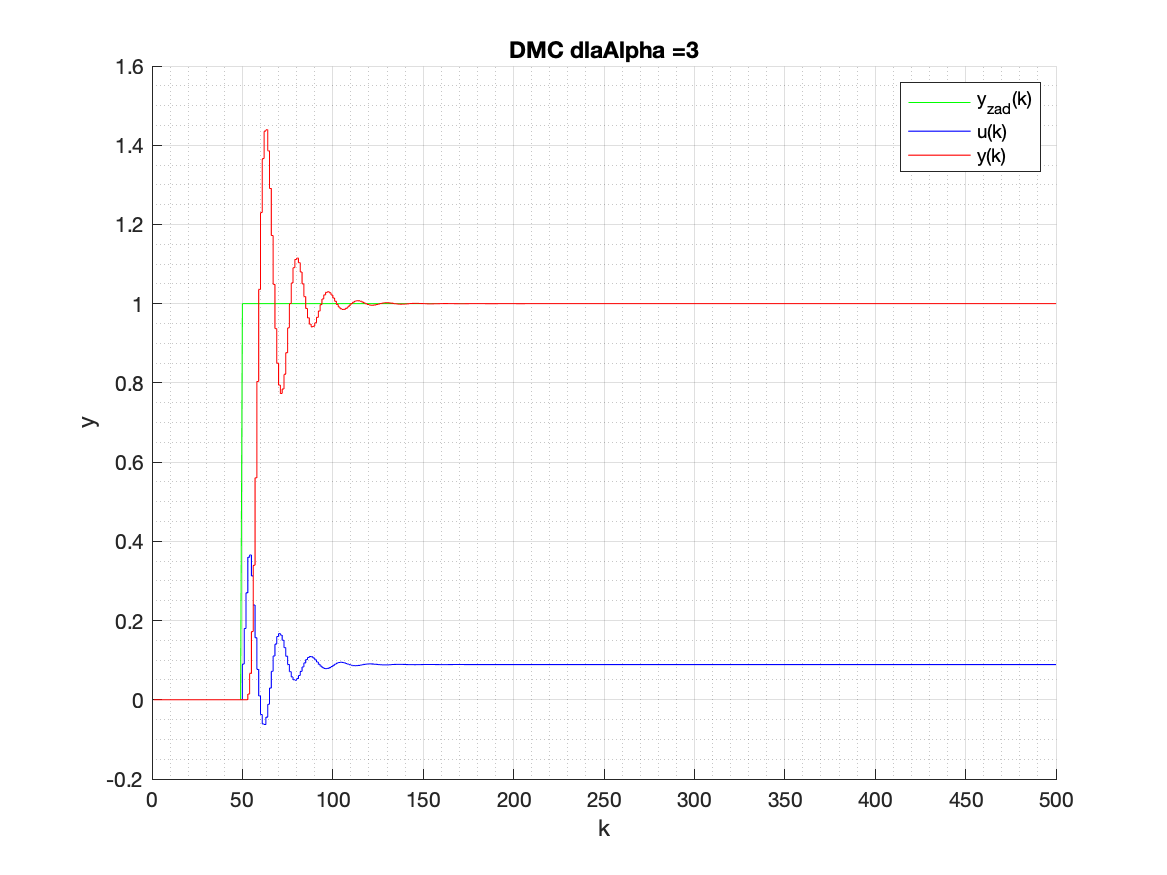
\includegraphics[width=\linewidth]{./ModelsDodatkowe_Alpha/P4_DMC_Alpha_3_png.png} 
 \includegraphics[width=\linewidth]{./ModelsDodatkowe_Alpha/P4_DMC_Alpha_3_6_png.png} 
 \includegraphics[width=\linewidth]{./ModelsDodatkowe_Alpha/P4_DMC_Alpha_4_2_png.png} 
 \includegraphics[width=\linewidth]{./ModelsDodatkowe_Alpha/P4_DMC_Alpha_4_3_png.png} 
 \includegraphics[width=\linewidth]{./ModelsDodatkowe_Alpha/P4_DMC_Alpha_4_4_png.png} 
 \includegraphics[width=\linewidth]{./ModelsDodatkowe_Alpha/P4_DMC_Alpha_5_4_png.png} 
 \includegraphics[width=\linewidth]{./ModelsDodatkowe_Alpha/P4_DMC_Alpha_8_9_png.png} 
 \includegraphics[width=\linewidth]{./ModelsDodatkowe_Alpha/P4_DMC_Alpha_10_png.png} 
 \newpage
 
 Przeprowadziłem także ten sam eksperyment ale dla DMC bez ograniczeń. System był odrobinę bardziej odporny na zmienność układu ale w ostateczności poddał się po wartości \( \alpha = 4.8\)
  
 \includegraphics[width=\linewidth]{./ModelsDodatkowe_AlphaNoOgr/P4_DMC_AlphaNoOgr_1_1_png.png} 
 
 \includegraphics[width=\linewidth]{./ModelsDodatkowe_AlphaNoOgr/P4_DMC_AlphaNoOgr_1_5_png.png} 
 \includegraphics[width=\linewidth]{./ModelsDodatkowe_AlphaNoOgr/P4_DMC_AlphaNoOgr_2_png.png} 
 \includegraphics[width=\linewidth]{./ModelsDodatkowe_AlphaNoOgr/P4_DMC_AlphaNoOgr_2_4_png.png} 
 
 \includegraphics[width=\linewidth]{./ModelsDodatkowe_AlphaNoOgr/P4_DMC_AlphaNoOgr_3_png.png} 
 \includegraphics[width=\linewidth]{./ModelsDodatkowe_AlphaNoOgr/P4_DMC_AlphaNoOgr_3_6_png.png} 
 \includegraphics[width=\linewidth]{./ModelsDodatkowe_AlphaNoOgr/P4_DMC_AlphaNoOgr_4_2_png.png} 
 \includegraphics[width=\linewidth]{./ModelsDodatkowe_AlphaNoOgr/P4_DMC_AlphaNoOgr_4_3_png.png} 
 \includegraphics[width=\linewidth]{./ModelsDodatkowe_AlphaNoOgr/P4_DMC_AlphaNoOgr_4_4_png.png} 
 \includegraphics[width=\linewidth]{./ModelsDodatkowe_AlphaNoOgr/P4_DMC_AlphaNoOgr_5_4_png.png} 
 \includegraphics[width=\linewidth]{./ModelsDodatkowe_AlphaNoOgr/P4_DMC_AlphaNoOgr_8_9_png.png} 
 \includegraphics[width=\linewidth]{./ModelsDodatkowe_AlphaNoOgr/P4_DMC_AlphaNoOgr_10_png.png} 
\end{enumerate}
\end{document}

